\chapter{Appendix}
\label{cha:appendix}

\section{Further Empirical Evaluation}

\begin{figure}[H]
     \centering
     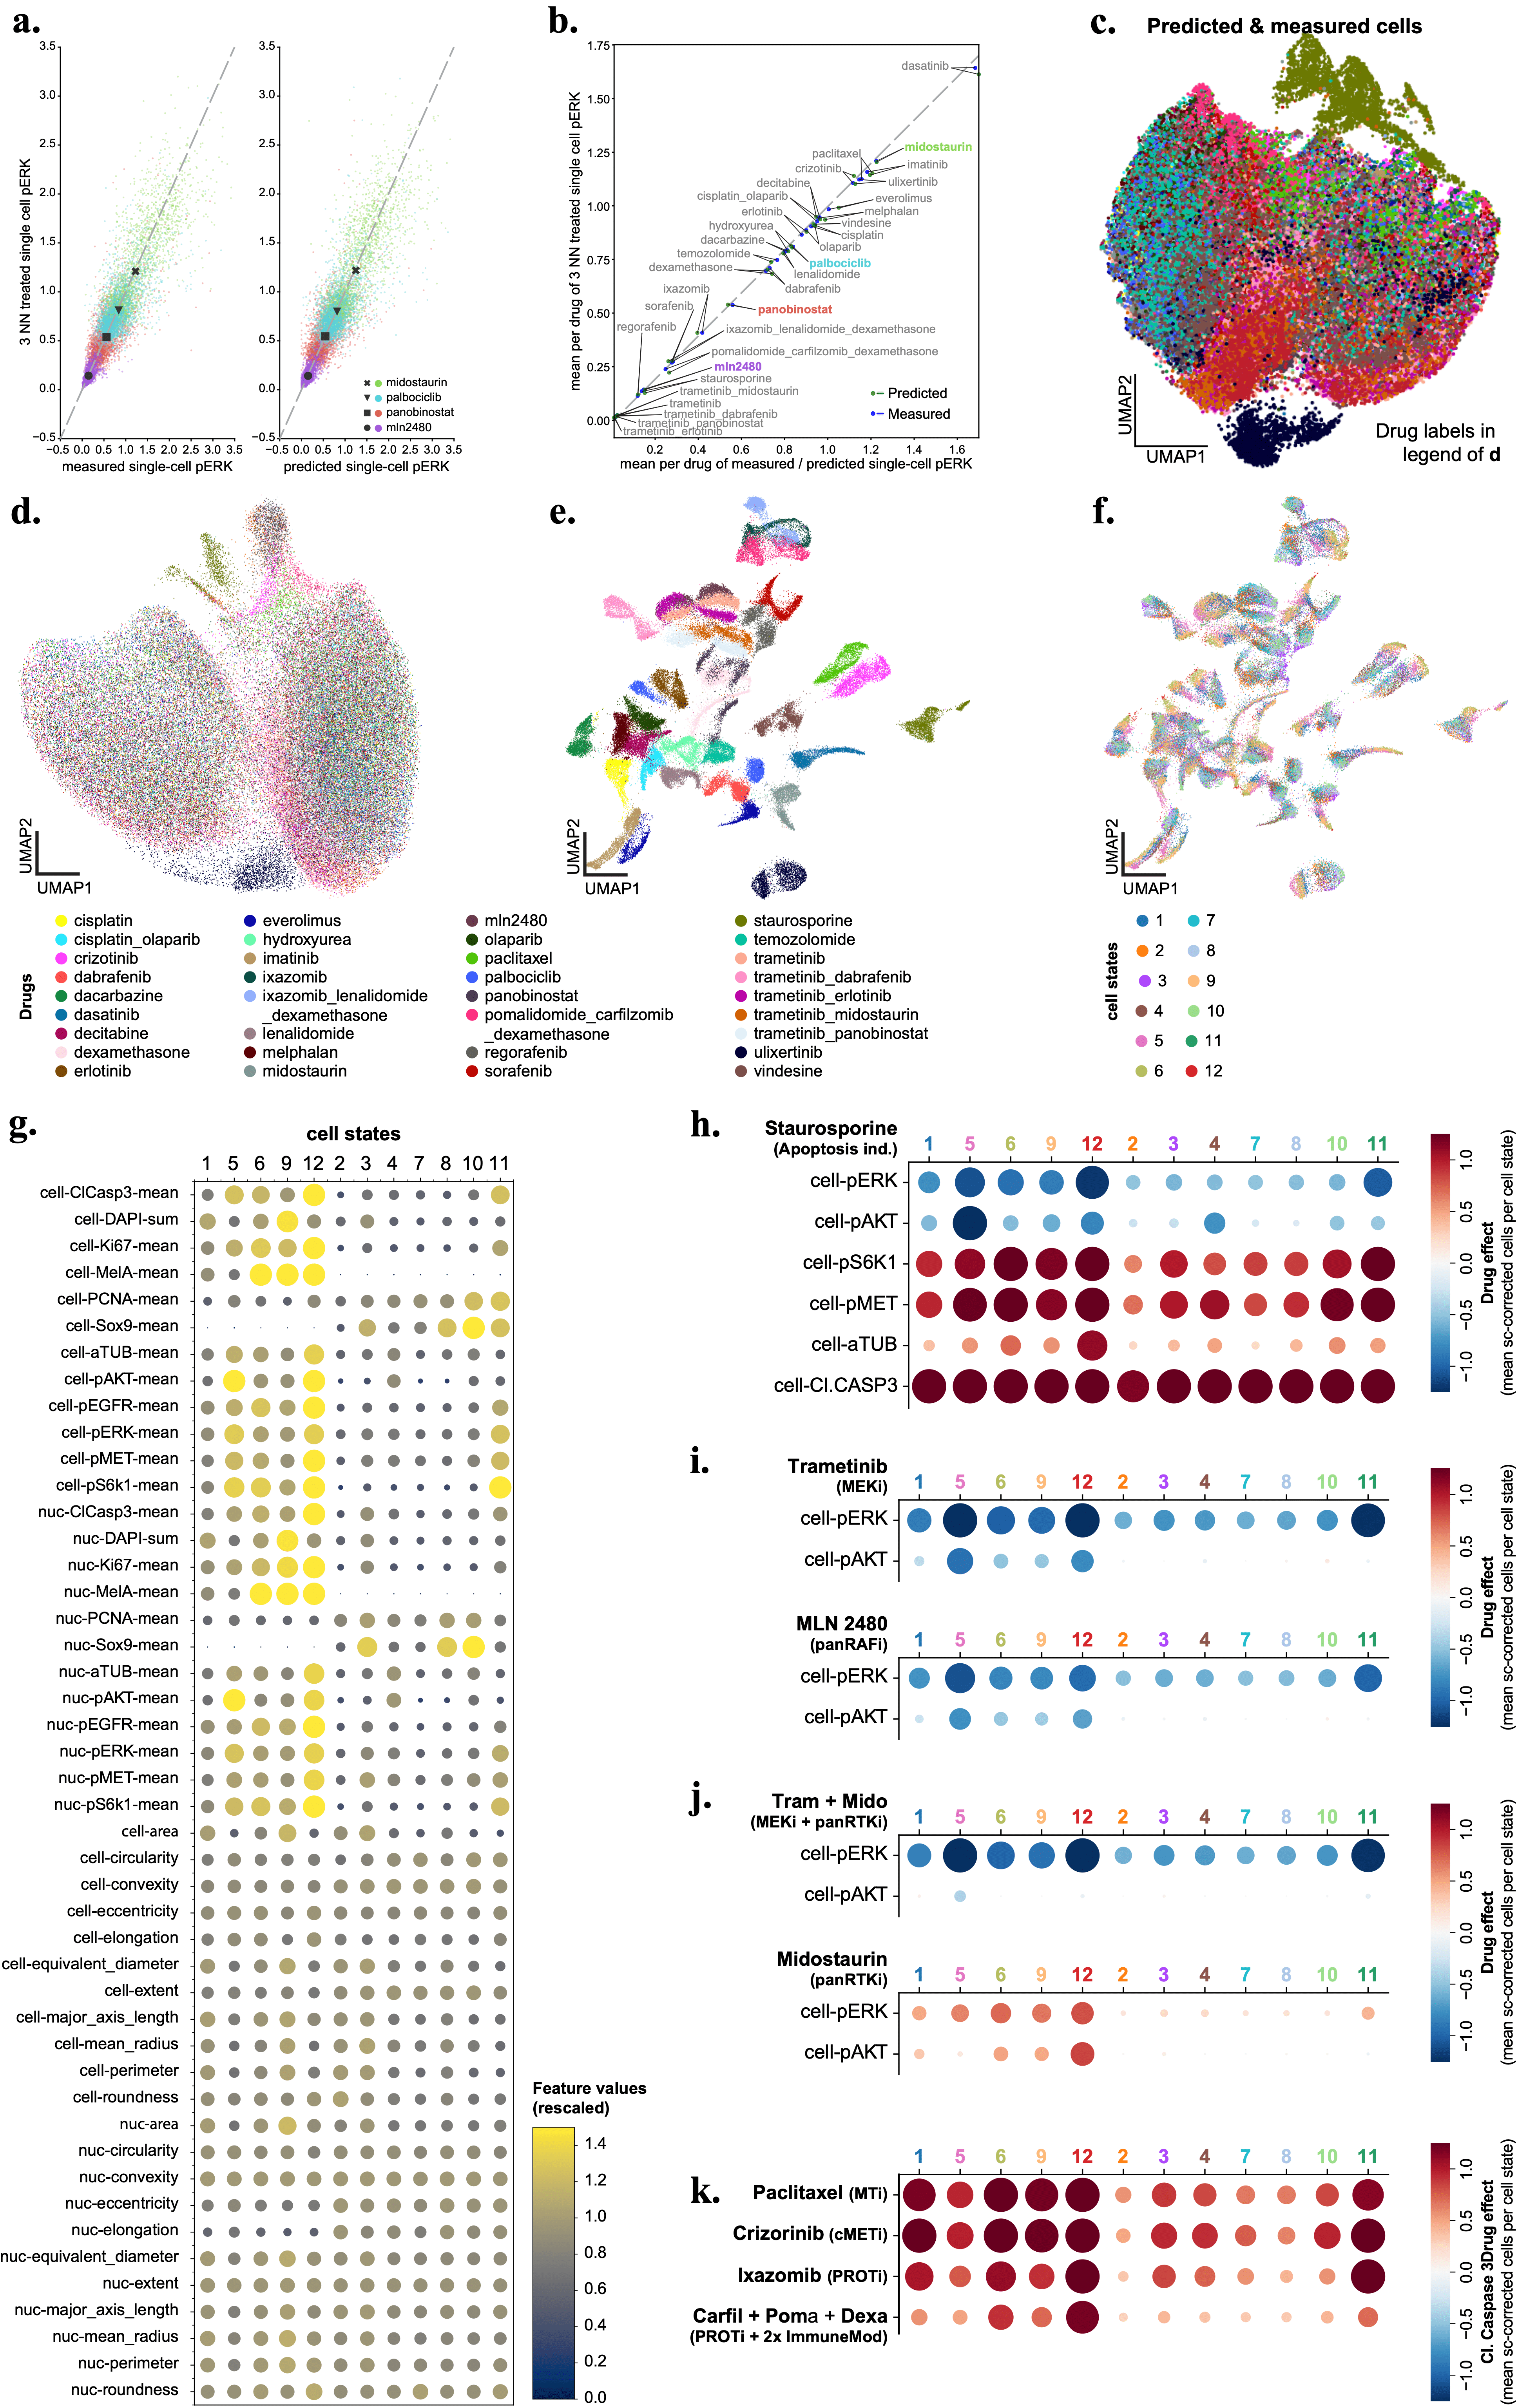
\includegraphics[height=.95\textheight ]{figures/fig_4i_analysis_extended.pdf}
\end{figure}
\captionof{figure}{
\textbf{a.} High similarity of measured and CellOT-predicted single-cell pERK (phosphor ERK1/2) values at the single-cell level. Scatter plots compare the relationship between measured pERK values of cells (left) treated with Midostaurin (green dots), Palbociclib (blue dots), Panobinostat (red dots), and MLN2480 (purple dots) or (right) predicted for those drugs along the horizontal axis to their corresponding 3NN cells on the vertical axis. X mark, square, inverted triangle, and circle represent the mean of the respective measurements per drug. The dashed gray line indicates the diagonal along which the measurements would correlate perfectly. \textbf{b.} The high similarity of measured and CellOT-predicted single-cell pERK (phosphor ERK1/2) values at the population level across all drug perturbations. Drug average of measured (blue dots) and predicted (green dots) pERK values compared to their respective 3NN measurement. Drug treatments highlighted in color correspond the those presented in panel \textbf{a.}. The dashed gray line indicates the diagonal along which the measurements would correlate perfectly. \textbf{c.} Projection of measured perturbed and predicted perturbed cells in a shared UMAP space. Each cell is color-coded according to the perturbation from which it originates. \textbf{d.} Projection of mean-corrected measured perturbed cells in a UMAP space. Each cell is color-coded according to the perturbation from which it originates. A mean correction was achieved by subtracting calculating the mean of every feature for all cells in the control condition and subtracting the calculated feature means from the feature values of individual cells. \textbf{e.} Projection of single-cell corrected, predicted perturbed cells in a UMAP space. Each cell is color-coded according to the perturbation model with which it was predicted. \textbf{f.} Projection of single-cell corrected, predicted perturbed cells in a UMAP space. Each cell is color-coded according to its assignment to one of the 12 cell states. \textbf{g.} Feature value overview of the 12 identified cell states in DMSO-treated (control) cells. Each column represents a cell state, and each row a feature. Circles are colored and scaled based on feature value, from small size in blue for low feature values, to large circles in yellow for high feature values. \textbf{h-j.} Drug effect overview of the 12 identified cell states in \textbf{h.} Staurosporine (apoptosis ind.m apoptosis inducer, \textbf{i.} Trametinib (MEKi, MEK inhibitor), MLN2480 (panRAFi, panRAF inhibitor), \textbf{j.} Trametinib + Midostaurin (Tram + Mido, MEK inhibitor + pan Receptor Tyrosine Kinase inhibitor (panRTK)), Midostaurin (panRTK). Each column represents a cell state, and rows represent features. "cell-" stands for mean cell intensity. Circles are scaled based on drug effect, the larger the $\pm$ effect the larger the circles. Negative values are encoded in hues of blue, and positive values in red hues of the respective circles. \textbf{k.} Effect of drug treatments on levels of cleaved Caspase 3 (cleaved Caspase 3) in the 12 identified cell states. Each column represents a cell state, and each row a drug treatment.}
\label{fig:4i_analysis_extended}

\newpage
\begin{figure}[H]
     \centering
     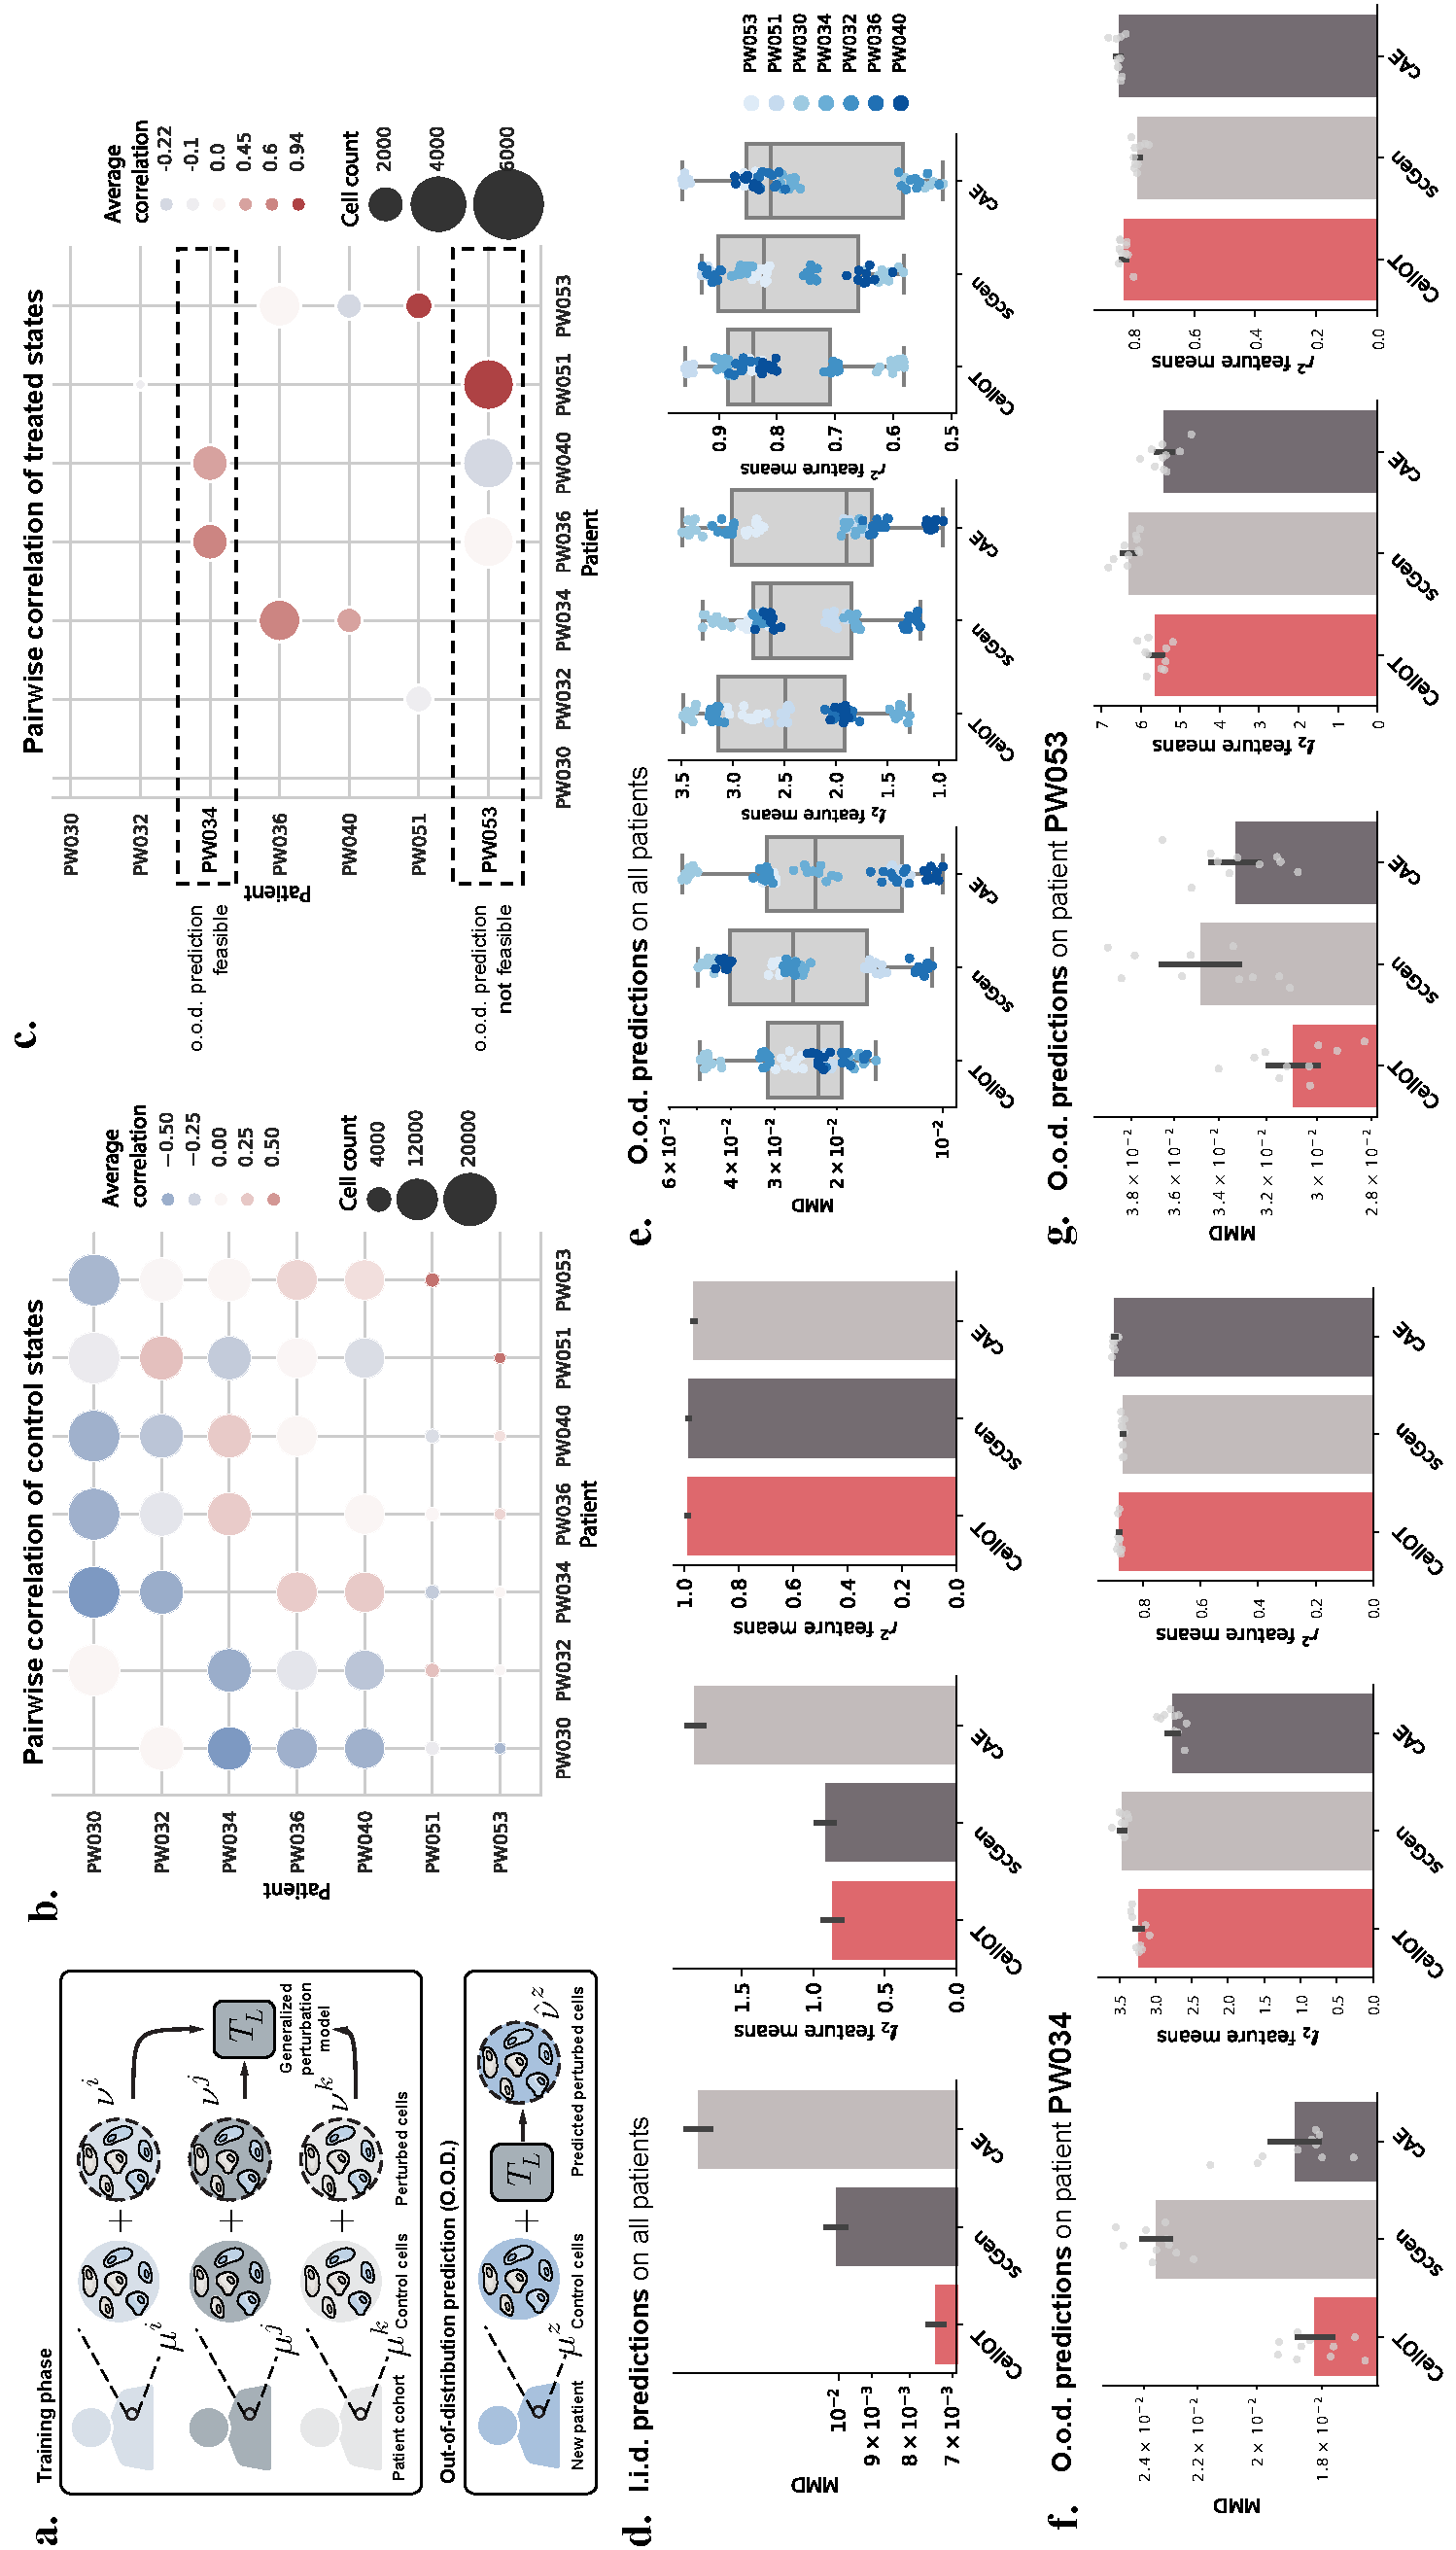
\includegraphics[width=0.8\textwidth]{figures/fig_gbm_patients_iid_ood.pdf}
\end{figure}
\captionof{figure}{Analysis and results of the glioblastoma dataset consisting of seven patients. \textbf{a.} Cells from seven glioblastoma patients are measured in an untreated and Panobinostat-treated state. For each sample, we train two models, an o.o.d.~model trained on cells from all other samples but the holdout patient we test on and an i.i.d.~model trained with additional access to half of the cells in the holdout sample.
    \textbf{b.} Pairwise average correlation of the PCA embeddings of the control states between patients. \textbf{c.} Pairwise average correlation of the PCA embeddings of the treated states between patients, masked to only those patient pairs that showed a positive correlation in the control states. Only patient PW034 positively correlates with all other patients. Other patients, such as PW053, correlate and anti-correlate with other patients in the treated state. Performance comparison between \textsc{CellOT} and baselines for different metrics in the \textbf{d.} i.i.d. setting (mean standard deviation across 7 samples, 10 bootstraps of the test set per sample),
    \textbf{e.} o.o.d. setting for all patients (box plots show median, minima, and maxima)
    \textbf{f.} o.o.d. setting for a patient positively correlating with all patients that are also similar in the control state,
    \textbf{g.} o.o.d. setting for a patient where similar patients in the control state show different responses (correlation and anti-correlation) in the treated states. Data in \textbf{f} and \textbf{g} are presented as the mean +/- standard deviation across n=10 bootstraps of the test set.}
\label{fig:gbm_patients_iid_ood}

\clearpage
\newpage

\begin{figure}[H]
     \centering
     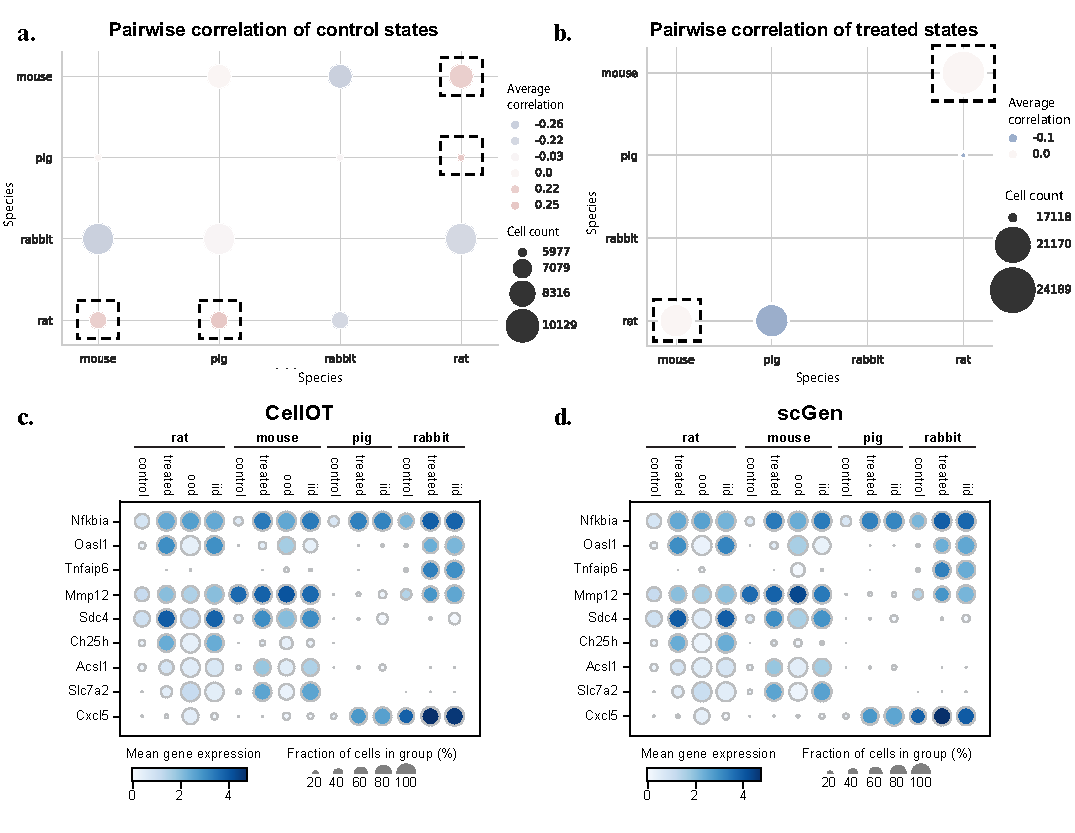
\includegraphics[width=\textwidth]{figures/fig_crossspecies_ood_analysis.pdf}
     \caption{\looseness -1 Analysis and further results of the cross-species dataset. \textbf{a.} Pairwise average correlation of the PCA embeddings of the control states between species. \textbf{b.} Pairwise average correlation of the PCA embeddings of the treated states between patients, masked to only those patient pairs that showed a positive correlation in the control states. Only rat and mouse show consistent responses, i.e., a positive correlation of the control states and a non-negative correlation of the respective target cells, and are thus chosen for the o.o.d. analysis. I.i.d. and o.o.d. results measured in the average gene expression for both \textbf{d.} \textsc{CellOT} and \textbf{c.} \textsc{scGen}.}
     \label{fig:crossspecies_ood_analysis}
\end{figure}

\section{Datasets} \label{app:datasets}

We evaluate methods introduced in this thesis on different tasks, each consisting of a pair of source $\mu$ and target measure $\nu$.
In particular, we consider single-cell datasets in which populations of single cells have been monitored with modern high-throughput methods such as single-cell RNA sequencing or optical phenotyping technologies (see \cref{sec:tech_background}).
In the following, we introduce each dataset, describe preprocessing steps, feature selection, and data splits.

\subsection{\citet{srivatsan2020massively}}
\label{app:dataset_srivatsan}

\looseness -1 Cancer drugs reduce uncontrolled cell growth and proliferation by inhibiting DNA replication and RNA transcription as well as targeting proteins crucial for cancer progression. In doing so, they modulate downstream signaling cascades, affect cell growth and morphology, and alter gene expression profiles of single cells. 
\citet{srivatsan2020massively} conduct a scRNA-seq-based phenotyping screen of transcriptional responses to thousands of independent perturbations at single-cell resolution.
The measured cell population contains three well-characterized cancer cell lines, including A549, a human lung adenocarcinoma, K562, a chronic myelogenous leukemia, and MCF7, a mammary adenocarcinoma cell line.
Due to the different transcriptional profiles of each cancer cell line, drug compounds might cause divergent cellular responses in each subpopulation.
The dataset contains $17,565$ control cells as well as a varying number of cells perturbed by different drugs with different dosages, i.e., $10\,$nM, $100\,$nM, $1,000\,$nM, $10,000\,$nM.

\paragraph{Data preprocessing.}
The data is available for download in the \acrfull{GEO} database under accession number \href{https://www.ncbi.nlm.nih.gov/geo/query/acc.cgi?acc=GSM4150378}{GSM4150378}.
For data quality control and preprocessing, we follow the analysis of \citet{lotfollahi2021compositional}. The count matrix obtained from GEO consists of $581,777$ cells. The data were subset to half its size, with $290,888$ cells remaining after quality control for all $188$ different compounds. We proceeded with log-transformation and the selection of $1,000$ highly-variant genes using \texttt{scanpy} \citep{wolf2018scanpy}.

\paragraph{Feature selection.}
Single-cell RNA sequencing data is very high-dimensional, even after selecting $1,000$ highly-variant genes.
For the downstream analysis of how well the overall perturbation effect has been captured, we thus select the top $50$ marker genes, i.e., those genes which show strong differences between perturbed and unperturbed states. This analysis is conducted based on the \texttt{scanpy}'s function \texttt{rank\_genes\_groups}, setting unperturbed cells as reference ~\citep{wolf2018scanpy}. The influence of the number of considered marker genes on different evaluation metrics is further analyzed in \citet{bunne2021learning}.

\subsection{\citet{bunne2021learning}}
\label{app:dataset_bunne}

Besides sc\acrshort{RNA-seq}, optical phenotypic screens, e.g., multiplexing tools such as 4i \citep{gut2018multiplexed}, are able to capture meaningful features related to both the treatment response heterogeneity (e.g., the phosphorylation or dephosphorylation of a kinase in a signaling pathway) and the pre-existing cell-to-cell variability (e.g., protein levels related to different cellular states or cell cycle phases) which my determine treatment response. 
% Traditional high-content imaging datasets often need to compromise between features describing either the former or the latter and may thus struggle to provide sufficient information to pair treated and control cells accurately.
In order to derive a proof-of-concept study and test if the proposed methods are able to capture heterogeneous single-cell responses, we consider two co-cultured primary melanoma cell lines (M130219 and M130429), which were derived from the same melanoma patient from different body sites \citet{bunne2021learning}.
M130219 originates from a subcutaneous biopsy taken during treatment with Bimetinib (MEKi), whereas M130429 was derived from a bone autopsy one month after stopping said targeted therapy \citep{raaijmakers2015new}. Both cell lines share the same driver mutation (NRAS Q61R) but are phenotypically diverse. The cell lines were screened with $34$ different drugs, partially applied as combination therapies.

\paragraph{Data preprocessing.}
The cells were seeded in a 384-well plate, and allowed to settle and adhere overnight. Drugs and dimethyl sulfoxide as the vehicle control was added to the cells the next morning and incubated for 8 and 24 hours, respectively, after which the cells were fixed with paraformaldehyde. Subsequently, 6 cycles of 4i were performed, for which the images were acquired with an automated high-content microscope.
We utilized a mixture of two melanoma tumor cell lines (ratio 1:1) in order to image a total of $97,748$.

Consequently, the cell lines are also classed as two different melanoma subtypes due to, amongst others, differences in marker expression~\citep{raaijmakers2015new}: the former a mesenchymal subtype (SOX9$^+$, MelA$^-$), the latter a melanocytic subtype (Sox9$^-$, MelA$^+$).
$10,995$ cells were imaged in the DMSO-treated control state and the rest are treated with one of the $34$ cancer therapies. Between $2,000$ and $3,000$ cells are profiled per treatment.

All image analysis steps were performed by our in-house platform called \href{https://github.com/TissueMAPS}{\texttt{TissueMAPS}}. The steps included illumination correction \citep{snijder2012single}, alignment of images from different acquisition cycles using fast Fourier transform \citep{guizar2008efficient}, segmentation of nuclei and cell outlines \citep{stoeger2015computer},  as well cellular and nuclear measurements of intensity and morphology features using the \texttt{scikit-image} library \citep{van2014scikit}.

The extracted marker intensities and morphological features are then re-normalized to the same numerical scale by dividing each feature with its 75th percentile computed on control cells. Values are then transformed with a log1p ($x \xleftarrow{} \log(x + 1)$) function\footnote{\label{fnt:dataset_download} The dataset can be downloaded via \url{https://doi.org/10.3929/ethz-b-000609681}.}.

\paragraph{Feature selection.}
A total of 47 features are reported, 21 morphological features and 26 protein intensities.

\begin{figure}
    \centering
    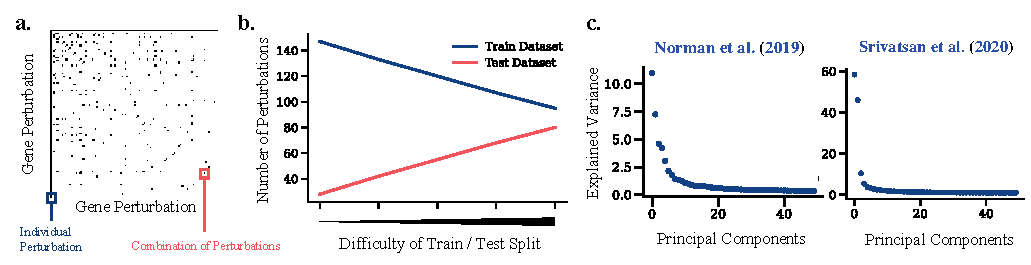
\includegraphics[width=.9\textwidth]{figures/fig_datasets_splits_processing.pdf}
    \caption{\textbf{a.} The indicator matrix of all individual perturbations as well as those perturbation pairs available in combination (black) in the dataset by \citet{norman2019exploring}. \textbf{b.} Size of the different train/test splits of the dataset by \citet{norman2019exploring}. The train set contains all single perturbations as well as a decreasing number of combinations with increasing difficulty of the data split. For more details, see \cref{app:datasplits}.}
    \label{fig:datasets_processing}
\end{figure}

\subsection{\citet{norman2019exploring}} 
\label{app:dataset_norman}

\looseness -1 Genetic interactions and their joint expression give rise to an inconceivable organismal complexity and uncountable many diverse phenotypes and behaviors.
Constructing a systematic genetic interaction map is crucial for a better understanding of cellular mechanisms in health and disease.
Thus, \citet{norman2019exploring} conducted single-cell, pooled transcriptional profiling of CRISPR-mediated perturbations to link genetic perturbation to its transcriptional consequences using the Perturb-Seq technology \citep{dixit2016perturb}.
The dataset consists of individual perturbations as well as joint overexpression of different genes, allowing us to study the phenotypic consequences of perturbing a pair of genes alone or in combination. The indicator matrix of all individual perturbations as well as those pairs available in combination can be found in \cref{fig:datasets_processing}a.

\paragraph{Data preprocessing.}
\looseness -1 The data is available for download in the \acrshort{GEO} database under accession number \href{https://www.ncbi.nlm.nih.gov/geo/query/acc.cgi?acc=GSE133344}{GSE133344}.
For data quality control and preprocessing, we follow the analysis of \citet{lotfollahi2021compositional}.
We discarded those genetic perturbations with less than $250$ cells, resulting in a dataset with $92$ individual perturbations and $84$ perturbations in combination.
This further included, the exclusion of particular subsets of control cells with in total of $98,419$ remaining, data normalization, log-transformation, and selection of $1,500$ highly-variant genes using \texttt{scanpy} \citep{wolf2018scanpy}.

\paragraph{Feature selection.}
Similar to \cref{app:dataset_srivatsan}, for evaluation we select the top $50$ marker genes, i.e., those genes most strongly affected by the particular genetic perturbation.

\paragraph{Data splits.} \label{app:datasplits}
For the evaluation conducted in \cref{cha:condot}, we create different train/test dataset splits of increasing difficulty by following \citet{lotfollahi2021compositional}.
The train splits hereby always contain all $92$ individual perturbations as well as varying numbers of combinations. The easiest train split contains 55 perturbations, while the test set only carries 28 combinations that are unknown in the evaluation. Consecutive splits get increasingly harder, comprising 42, 29, 16, and 4 combinations in the train set (besides all single perturbations) and 41, 54, 67, and 79 combinations in the test set, respectively (see \cref{fig:datasets_processing}b).

\subsection{\citet{moon2019visualizing}}
\label{app:dataset_moon}

Developmental processes in biology involve tissue and organ development, body axis formation, cell division, and cell differentiation, e.g., the development of stem cells into functional cell types.
An example of such a process is the differentiation of \acrshort{ESC} into  hematopoietic, cardiac, neural, pancreatic, hepatocytic, and germ lineages.
This development can be approximated \textit{in vitro} using \acrfull{EB} \citep{martin1975differentiation}, three-dimensional aggregates of pluripotent stem cells, including ESCs \citep{shamblott2009derivation}.
Recently, \citet{moon2019visualizing} conducted a scRNA-seq analysis to unveil the developmental trajectories, as well as cellular and molecular identities through which early lineage precursors emerge from human ESCs.
The dataset is available via \href{https://data.mendeley.com/datasets/v6n743h5ng}{Mendeley Data (V6N743H5NG)}\footnote{Dataset available via \url{https://data.mendeley.com/datasets/v6n743h5ng}.}.
In the following, we describe the preprocessing of the raw scRNA-seq data as well as the lineage branch analysis extracting the functional cell types emerging in this developmental process.

\paragraph{Data preprocessing.}
To preprocess the data, we follow the analysis of \citet{moon2019visualizing} as well as \citet{luecken2019current}. \citet{moon2019visualizing} originally measure  approximately $31,000$ cells over a 27 days differentiation time course, comprising gene expression matrices and barcodes, i.e., DNA tags used to identify reads originating from the same cell. The measured cells are then filtered in a quality control stage, their gene expression levels normalized and further processed in a feature selection step, where only highly-differentiated genes are selected.
After quality control, the dataset consists of $15,150$ cells and $17,945$ genes.

\paragraph{Feature selection.}
We extract $4,000$ \acrfull{HVG} using the 10X genomics preprocessing software \texttt{Cell Ranger} \citep{zheng2017massively} to further reduce the dimensionality of the dataset and include only the most informative genes.
Given the resulting data matrix with $15,150$ cells and $4,000$ genes across 5 different time points, we compute a corresponding low-dimensional embedding using PCA. We use the first 20 or 30 PCs for predicting population dynamics in \cref{cha:neural_pde} and \ref{cha:neural_sde}.
This is in alignment with previous analysis of developmental trajectories, which use 5 \citep{tong2020trajectorynet} and 30 PCs \citep{schiebinger2019optimal}, respectively.

\paragraph{Lineage branch analysis.}
Besides evaluating how well methods presented in this thesis resemble the spatiotemporal dynamics, we analyze their ability to capture biological heterogeneity.
Serving as an \emph{in vitro} model of early embryogenesis, embryoid bodies differentiation captures the development of \acrshortpl{ESC} into the mesoderm, endoderm, neuroectoderm, neural crest, and others.
Using an initial $k$-means clustering ($k=30$) and following \citet[Fig. 6, Suppl. Note 4]{moon2019visualizing}, we compute lineage branch classes for all cells in a 10-dimensional embedding space using PHATE, a non-linear dimensionality reduction method capturing a denoised representation of both the local and global structure of a dataset.
Details of the annotation can be found in \citet{bunne2022proximal, bunne2022recovering}.

We then train a $k$-NN classifier ($k=5$) to infer the lineage branch class based on a 30-dimensional PCA embedding of a cell (ESC: 0, neural crest: 1, neuroectoderm: 2, endoderm: 3, mesoderm: 4, other: 5).
\cref{sec:jkonet_cell} and \ref{sec:gsbflow_cell} thereby contains an analysis of the captured lineage branch heterogeneity of the predictions by computing the lineage branch class of each cell using the $k$-NN classifier.

\subsection{\citet{weinreb2020lineage}}
\label{app:dataset_weinreb}

\citet{weinreb2020lineage} study lineage tracing on transcriptional landscapes in hematopoiesis, the process of blood regeneration in bone marrow, in which multipotent progenitors give rise to red cells of the blood, as well as myeloid and lymphoid immune cell types.
In order to dissect how molecular differences among progenitor cells determine their ability to generate mature cell types, it is crucial to understand the hierarchy of fate decisions connecting stem and progenitor cells through time.
Directly linking whole-transcriptome descriptions of cells to their future fate is challenging, however, as single-cell \acrshort{RNA-seq} technologies are destructive (see \cref{sec:tech_background}). 
\citet{weinreb2020lineage} therefore clonally tag cells with DNA barcodes that can be read using sc\acrshort{RNA-seq} and enable tracing cellular identities through time.
The resulting dataset consists of three snapshots taken on days 2, 4, and 6, respectively. While at day 2 most cells are undifferentiated, at later time points cells have developed into neutrophils, monocytes, megakaryocytes, mast cells, lymphoid precursors, erythrocytes, basophils, eosinophils, etc.

\paragraph{Data preprocessing.}
The data used in \cref{cha:cellot} and \cref{sec:sbalign} is available for download in the \acrshort{GEO} database under accession number \href{https://www.ncbi.nlm.nih.gov/geo/query/acc.cgi?acc=GSE140802}{GSE140802}.
For data quality control and preprocessing, we follow the analysis of \citet{lotfollahi2021compositional}, resulting in a dataset containing $130,861$ cells.
After processing, each observation records the level of expression of $1,622$ different highly-variable genes as well as the following metainformation per cell:
\begin{itemize}
    \item a \texttt{timestamp}, expressed in days and taking values in \{2, 4, 6\},
    \item a \texttt{barcode}, which is a short DNA sequence that allows tracing the identity of cells and their lineage by means of single-cell sequencing readouts,
    \item an additional \texttt{annotation}, which describes the current differentiation fate of the cell.
\end{itemize}

For experiments conducted in \cref{sec:sbalign_cell}, we only retain cells with barcodes that appear both on days 2 and 4, taking care of excluding cells that are already differentiated on day 2.
We construct matchings by pairing cells measured at two different times but which share the barcode. 
Additionally, we filter cells to make sure that no one appears in more than one pair.

\paragraph{Feature selection.}
To reduce the dimensionality of these data points, we perform a PCA projection down to 50 components.

\subsection{Other Datasets}
\label{app:dataset_other}

Preprocessing for the lupus patients~\citep{kang2018multiplexed} and cross-species dataset~\citep{hagai2018gene} were inherited from~\citet{rybakov2020learning} 
and \citet{lotfollahi2019scgen}, and we would like to thank the authors for hosting this dataset.
Lastly, the preprocessing of the glioblastoma patient dataset \citep{zhao2021deconvolution} was adapted from \citet{peidli2022scperturb}.
The preprocessed datasets are available for download\textsuperscript{\ref{fnt:dataset_download}}.

\section{Evaluation Metrics} \label{app:evaluation_metrics}

\looseness -1 Since we lack access to the ground truth pair of perturbed and unperturbed observations on the single cell level, we consider evaluation metrics on the level of the distribution of real and predicted perturbation states to analyze the effectiveness of the approaches presented in this thesis.

\paragraph{Average- and Correlation-based distance.} 
Common evaluation metrics in single-cell biology rely on averages and correlation analysis. $\ell_2$ feature means thereby refers to the $\ell_2$-distance between means of the observed and predicted distributions. Similarly, $r_2$ feature means refers to the correlation of the means of the observed and predicted distributions.
However, metrics based only on feature means can be insensitive in settings where crucial heterogeneity is not captured. Consider, for example, a target distribution with multiple modes. These metrics will favorably evaluate a uni-modal predicted distribution that simply models the mean of this multi-modal distribution. To this end, we include a distributional distance sensitive to this type of behavior by measuring differences in the properties of higher moments, i.e., the maximum mean discrepancy.
We thus also report results based on several distributional metrics:

\paragraph{Wasserstein distance.}
We measure accuracy of the predicted target population $\hat{\nu}$ to the observed target population $\nu$ using the entropy-regularized Wasserstein distance \citep{cuturi2013sinkhorn} provided in the \texttt{OTT} library \citep{cuturi2022optimal} introduced in \cref{sec:background_kantorovich} and defined in \eqref{eq:ot-reg}.

\paragraph{Maximum mean discrepancy.}
Kernel maximum mean discrepancy~\citep{gretton2012kernel} is another metric to measure distances between distributions, i.e., for our purpose between the predicted target population $\hat{\nu}$ to the observed target population $\nu$.
Given two random variables $x$ and $y$ with distributions $\hat{\nu}$ and $\nu$, and a kernel function $\omega$, \citet{gretton2012kernel} define the squared MMD as:
\begin{equation*}
    \text{MMD}(\hat{\nu},\nu; \omega) = \mathbb{E}_{x,x^\prime}[\omega(x, x^\prime)] + \mathbb{E}_{y,y^\prime}[\omega(y, y^\prime)] - 2\mathbb{E}_{x,y}[\omega(x, y)].
\end{equation*}
We report an unbiased estimate of $\text{MMD}(\hat{\nu},\nu)$, in which the expectations are evaluated by averages over the population particles in each set. We utilize the RBF kernel, and as is usually done, report the MMD as an average over several length scales, i.e., \texttt{np.logspace(1, -3)}.

\paragraph{Perturbation signatures.}
A common method to quantify the effect of a perturbation on a population is to compute its perturbation signature \citep[(PS)]{stathias2018drug}, computed via the difference in means between the distribution of perturbed states and control states of each feature, e.g., here individual genes. $\ell_2$(PS) then refers to the $\ell_2$-distance between the perturbation signatures computed on the observed and predicted distributions, $\nu$ and $\hat{\nu}$. As before, let $\mu$ be the set of observed unperturbed population particles, $\nu$ the set of observed perturbed particles, as well as $\hat{\nu}$ the predicted perturbed state of population $\mu$. The $\ell_2$(PS) is then defined as
\begin{equation*}
    \text{PS}(\nu, \mu) = \frac{1}{m}\sum_{y_i \in \nu}{y_i} - \frac{1}{n}\sum_{x_i \in \mu}{x_i},
\end{equation*}
where $n$ is the size of the unperturbed and $m$ of the perturbed population.
We report the $\ell_2$ distance between the observed signature $\text{PS}(\nu, \mu)$ and the predicted signature $\text{PS}(\hat{\nu}, \mu)$, which is equivalent to simply computing the difference in the means between the observed and predicted distributions.


\numberwithin{equation}{section}		% for numbering  in the appendix
\numberwithin{lemma}{section}		% for numbering  in the appendix
\numberwithin{proposition}{section}		% for numbering  in the appendix
\numberwithin{theorem}{section}		% for numbering in the appendix

%----------------------------------------------------------------------
%%% PROOF OF BURES-WASSERSTEIN MECHANICS
%----------------------------------------------------------------------
\section{Proof of \cref{thm:gsbtobb}}
\label{app:gsbtobb}


It is known that, for \acrshortpl{SB}, the optimal solution can be searched within the class of stochastic processes \citep{leonard2013survey}
\begin{equation}
\label{eq:holddd}
X_t \sim \Pmargin: \quad\dd X_t =  (\driftf(X_t) + \vectalt(X_t) )\dt + \volat \dWiener[\ctime].
\end{equation}
The Fokker-Planck equation for the \acrshort{SDE} \eqref{eq:holddd} is
\begin{align}
\label{eq:FK}
\del_t \measure = - \Div \parens*{  \measure(  \driftf +\vectalt  ) } + \frac{\volatsq[\ctime]}{2}\Laplace \measure.
\end{align}
A simple application of the Girsanov theorem then shows, up to a constant, 
\begin{align}
\label{eq:KLobj}
\KL(\Pmargin \| \refsde) = \exof*{ \int_0^\horizon\frac{\norm{\vectalt}^2}{2\volatsq[\ctime]}   \dt}.
\end{align}
Using a change of variable $\vect = \vectalt - \frac{\volatsq[\ctime]}{2}\nabla\log\measure$, we see that \eqref{eq:FK} is equivalent to
\begin{equation}
\del_t \measure = - \Div \parens*{  \measure(  \driftf +\vect  ) }.
\end{equation}
On the other hand, since $\norm{\vectalt}^2 = \norm{\vect}^2 + \frac{\volat^4}{4}\norm*{\nabla\log\measure}^2 + 2 \inner*{\vect}{ \frac{\volatsq[\ctime]}{2}\nabla\log\measure}$, the integrand in the objective of \eqref{eq:KLobj} becomes 
\begin{align}
 \mathbb{E}\Bigg[\int_0^\horizon  \frac{\norm{\vect}^2}{2\volatsq[\ctime]} + \frac{\volatsq[\ctime]}{8} \norm{\nabla \log \measure}^2  + \frac{1}{2} \inner{\vect}{\nabla \log\measure} \dt\Bigg].
\end{align}


Letting $H(\measure) \defeq \int \measure\log\measure$ be the entropy, we have
\begin{align*}
H(\measure[\horizon]) - H(\measure[0]) &= \int_0^\horizon \del_t H(\measure) \dt \\
&= \int_0^\horizon  \int   (1+ \log\measure) \del_t\measure \drm \point \dt  \\
&= \int_0^\horizon  \int   (1+ \log\measure) \cdot \parens*{ - \Div \parens*{ \measure(\driftf+\vect) }  } \drm \point \dt  \quad\quad \text{by \eqref{eq:FK}}\\
&= \int_0^\horizon  \int   \measure \inner{\nabla\log\measure}{ \driftf+\vect} \drm \point \dt 
\end{align*}
by integration by parts for the divergence operator. Therefore,
\begin{align}
\exof*{\int_0^\horizon  \inner{\nabla\log\measure}{ \vect}  \dt } = H(\measure[\horizon]) - H(\measure[0])-\exof*{\int_0^\horizon  \inner{\nabla\log\measure}{ \driftf}  \dt }
\end{align} 
which concludes the proof.\qed



%----------------------------------------------------------------------
%%% PROOF OF BURES-WASSERSTEIN MECHANICS
%----------------------------------------------------------------------
\section{The Bures-Wasserstein Geometry of Gaussian SBs}
\label{app:mechanics}

\subsection{Review of Bures-Wasserstein Geometry}

\label{app:reviewBW}

Recall that the \emph{metric tensor} $\innerBW[\cdot][\cdot][\Sigma]$ in the \emph{Bures-Wasserstein geometry} \citep{takatsu2010wasserstein} is defined in terms of the Lyapunov operator: 
\begin{align}
\label{eq:BW-tensor}
\forall\ U, V\in \tspace, \quad \innerBW[U][V][\Sigma] \defeq \tr\lyap[\Sigma][U]\Sigma\lyap[\Sigma][V] = \frac{1}{2}\tr \lyap[\Sigma][U]V.
\end{align}The corresponding Bures-Wasserstein norm is induced via $\normBWsq[U][\Sigma] \defeq \innerBW[U][U][\Sigma]$.
Another important operator is the Bures-Wasserstein \emph{gradient}: For any function $F \from \SPD \to \R$, 
\begin{equation}
\label{eq:gradBW-def}
\tspace\ni \gradBW F(\Sigma) \defeq 2 \parens*{ \nabla F(\Sigma)\Sigma + \Sigma \nabla F(\Sigma)^\top }
\end{equation}where $\nabla$ is the usual Euclidean gradient of $F$, viewed as a function from $\R^{\vdim\times\vdim}$ to $\R$. Note that
\begin{align}
\lyap[\Sigma][\gradBW F(\Sigma)] &= 2 \lyap[\Sigma][\nabla F(\Sigma)\Sigma + \Sigma\nabla F(\Sigma)] \\
&= 2 \nabla F(\Sigma)
\end{align}by definition of the Lyapunov operator. In other words,
\begin{align}
\label{eq:gradBW-lyapinv}
\gradBW F(\Sigma) = \lyapinv.
\end{align}


Lastly, we recall the Bures-Wasserstein \emph{acceleration} of a curve $\Sigcurve: [0,\horizon] \to \SPD$, which we denote by $\nabla_{\ssstyle\dSigcurve}\dSigcurve$:\footnote{More formally, $\nabla_{\ssstyle\dSigcurve}\dSigcurve$ is the Bures-Wasserstein covariant derivative of $\dSigcurve$ in the direction of $\dSigcurve$.}

\begin{align}
\label{eq:coderBW}
\coder = \ddSigcurve -  \parens*{  \lyap \dSigcurve + \dSigcurve\lyap } + \parens*{ \Sigcurve \parens*{\lyap}^2 + \parens*{\lyap}^2 \Sigcurve}.
\end{align}





\subsection{Proof of \cref{thm:mechanics}}
\label{app:proofmechanics}


For convenience, we restate \cref{thm:mechanics} in full below: 
\mechanics*


The proof consists of verifying the Euler-Lagrange equation \eqref{eq:el-bw} for the curve \eqref{eq:solMain}.

\subsubsection{Verifying the Euler-Lagrange Equation \eqref{eq:el-bw}}
\label{sec:verifyEL}
We begin by noting that the boundary conditions in \eqref{eq:el-bw} hold for the curve in \eqref{eq:solMain}. 


We now compute the two sides of \eqref{eq:el-bw} separately:

\paragraph{The right-hand side of \eqref{eq:el-bw}: $-\gradBW\penergyBW$.}
~Since $\nabla \penergyBW = -\nabla \parens*{\tr \frac{\sdev^4}{8} \Sigcurveinv} =  \frac{\sdev^4}{8} \Sigcurveinv\cdot \Sigcurveinv$, we see from \eqref{eq:gradBW-def} that the negative Bures-Wasserstein gradient of $\penergyBW$ is
\begin{align}
\nn
-\gradBW \penergyBW &= -2\parens*{\frac{\sdev^4}{8} \Sigcurveinv\cdot \Sigcurveinv \cdot \Sigcurve + \Sigcurve\cdot \frac{\sdev^4}{8} \Sigcurveinv\cdot \Sigcurveinv } \\
\label{eq:gradBWU}
&= -\frac{\sdev^4}{2} \Sigcurveinv.
\end{align}


\paragraph{The left-hand side of \eqref{eq:el-bw}: $\coder$.}
~Computing $\coder$ is significantly trickier than $-\gradBW\penergyBW$. The central piece of the proof is the following technical lemma:
\begin{lemma}
\label{lem:lyap}
Define the matrix $\Ht$ to be:
\begin{equation}
\label{eq:Ht}
\Ht \defeq \ctime\Sigma\prime + \ctimebar \C - \ctimebar\Sigma - \ctime\C^\top + \frac{\sdev^2}{2}(\ctimebar-\ctime)\eye.
\end{equation}Then $\lyap = \Ht^\top \Sigcurveinv$. In other words, $\Ht^\top \Sigcurveinv$ is symmetric and solves the Lyapunov equation:
\begin{equation}
  A: \quad  A\Sigcurve + \Sigcurve A= \dSigcurve.
\end{equation}
Moreover, $\Ht$ satisfies the following identity:
\begin{equation}
\label{eq:ht-id}
\dHt - \Sigcurveinv \Ht^2 =- \frac{\sdev^4}{4} \Sigcurveinv.
\end{equation}

\end{lemma}

Before commencing the proof of \cref{lem:lyap}, let us show how it readily leads us to \eqref{eq:el-bw}.

Recall the definition of $\coder$ in \eqref{eq:coderBW}. First, note that, by \eqref{eq:solMain} and \eqref{eq:Ht},
\begin{align}
\label{eq:ddot}
\frac{1}{2}\ddSigcurve &=   \Sigma+\Sigma\prime -  \parens*{  \C + \C^\top+ \sdev^2\eye }   \\
&=  \dHt.
\end{align}
On the other hand, \cref{lem:lyap} entails that
\begin{align}
\nn
\Sigcurve \parens*{\lyap}^2 + \parens*{\lyap}^2 \Sigcurve &= \Sigcurve \lyap \cdot \lyap + \lyap \cdot \lyap\Sigcurve \\
\nn
 &= \Sigcurve \Sigcurveinv \Ht \cdot \lyap + \lyap \cdot \Ht^\top \Sigcurveinv \Sigcurve \\
 \label{eq:holdBW}
 &= \Ht \lyap + \lyap \Ht^\top.
\end{align}
By noting, again from \cref{lem:lyap},
\begin{align}
\nn
\dSigcurve &= \Ht^\top \Sigcurveinv \cdot \Sigcurve + \Sigcurve \cdot \Sigcurveinv\Ht \\
\label{eq:HtHtt}
&= \Ht + \Ht^\top,
\end{align}
we thus get
\begin{align}\nn
 \Sigcurve \parens*{\lyap}^2 &+ \parens*{\lyap}^2 \Sigcurve- \parens*{  \lyap \dSigcurve + \dSigcurve\lyap } \\
 &= \parens*{\Ht - \dSigcurve} \lyap + \lyap \parens*{\Ht^\top - \dSigcurve} \\
 \nn
 &= - \parens*{ \Ht^\top\lyap + \lyap \Ht  }
\end{align}by \eqref{eq:HtHtt}. But $\Ht^\top\lyap  = \Ht^\top \cdot \Sigcurveinv \Ht =\Sigcurveinv \Ht^2$ by symmetry of $\Ht^\top \Sigcurveinv$ and, similarly, we have $\lyap\Ht =  \Sigcurveinv \Ht^2$. As a result, \eqref{eq:coderBW} reduces to
\begin{align}
\label{eq:holdBW1}
\coder &= 2\dHt - 2 \Sigcurveinv\Ht^2.
\end{align}In lieu of \eqref{eq:el-bw}, \eqref{eq:gradBWU}, and \eqref{eq:holdBW1}, the proof of \eqref{eq:LagBW} can thus be reduced to showing
\begin{align}
2\dHt -  2\Sigcurveinv\Ht^2 = -\frac{\sdev^4}{2} \Sigcurveinv
\end{align}which is exactly \eqref{eq:ht-id}.



\begin{proof}[Proof of \cref{lem:lyap}] 
We now prove \cref{lem:lyap}. We begin by proving some useful identities that will inspire our proof for the general \acrshortpl{GSB} in \cref{sec:results_gsbflow}.

\paragraph{Useful identities.}
~First, note that the definition of $\C$ immediately implies $\C \Sigma = \Sigma \C^\top$. In addition, we have
\begin{align}
\nn
\C^{-1} \Sigma &= 2\parens*{ \Sigma^{\frac{1}{2}} \D  \Sigma^{-\frac{1}{2}} - \sdev^2\eye }^{-1} \Sigma \\
\nn
&= 2 \parens*{ \Sigma^{-\frac{1}{2}} \D  \Sigma^{-\frac{1}{2}} - \sdev^2\Sigma^{-1} }^{-1} \\
\label{eq:Csym}
&= \Sigma \C^{-\top}.
\end{align}
Recall from \citep{janati2020entropic} that $\C$ solves the following matrix equation:
\begin{align}
\label{eq:C}
\C^2 + \sdev^2\C =  \Sigma\Sigma\prime.
\end{align}
We therefore have
\begin{align*}
\C &= \C^{-1} \Sigma\Sigma\prime - \sdev^2\eye, \\
\C^\top &= \Sigma\prime\Sigma\C^{-\top} - \sdev^2\eye,
\end{align*}which, together with \eqref{eq:Csym}, implies
\begin{align}
\nn
\C^\top \Sigma\prime &= \Sigma\prime\Sigma \C^{-\top}\Sigma\prime-\sdev^2\Sigma\prime  \\
\nn
&=\Sigma\prime \C^{-1}\Sigma \Sigma\prime-\sdev^2\Sigma\prime   \\
\label{eq:Ctsym}
&= \Sigma\prime \C.
\end{align}


Now, set $\Ht = \Pt - \Qt^\top + \frac{\sdev^2}{2}(\ctimebar-\ctime)\eye$ where
\begin{align}
\Pt \defeq \ctime \Sigma\prime + \ctimebar \C, \quad \Qt \defeq \ctimebar \Sigma + \ctime \C.
\end{align}
Note that, by \eqref{eq:Ctsym}, 
\begin{align}
\nn
\Sigma\prime\Pt^{-1}  &= \parens*{ \Pt\Sigma\prime^{-1} }^{-1} \\
\nn
&= \parens*{\ctime\eye + \ctimebar  \C \Sigma\prime^{-1} }^{-1} \\
\nn
&=  \parens*{\ctime\eye + \ctimebar \Sigma\prime^{-1} \C^\top  }^{-1} \\
\nn
&= \parens*{ \Sigma\prime^{-1} \Pt^\top  }^{-1} \\
\label{eq:Ptsym}
&= \Pt^{-\top}\Sigma\prime.
\end{align}A similar calculation leading to \eqref{eq:Ptsym} shows
\begin{align}
\label{eq:Qtsym}
\Qt^{-1} \Sigma = \Sigma\Qt^{-\top}.
\end{align}

\paragraph{Proof of symmetry of $\Ht^\top\Sigcurveinv$.}
~We get, by \eqref{eq:C} and \eqref{eq:Ctsym},

\begin{align}
\nn
\Pt^2 + \sdev^2\ctimebar\Pt &= t^2 \Sigma\prime^2 + \ctimebar^2\C^2 + \ctime\ctimebar\parens*{ \Sigma\prime\C + \C\Sigma\prime } + \sdev^2 \ctime\ctimebar \Sigma\prime + \sdev^2\ctimebar^2 \C \\
\nn
&= t^2 \Sigma\prime^2 + \ctimebar^2 \parens*{ \C^2 + \sdev^2\C } + \ctime\ctimebar\parens*{ \C^\top\Sigma\prime + \C\Sigma\prime } + \sdev^2 \ctime\ctimebar \Sigma\prime\\
\label{eq:Pteq}
&= t^2 \Sigma\prime^2 + \ctimebar^2 \Sigma\Sigma\prime + \ctime\ctimebar\parens*{ \C^\top + \C + \sdev^2\eye}\Sigma\prime = \Sigcurve\Sigma\prime.
\end{align}

It then follows from \eqref{eq:Pteq} that

\begin{align}
\label{eq:Pt2}
\Pt &=  \Sigcurve\Sigma\prime\Pt^{-1} - \sdev^2 \ctimebar\eye, \\
\label{eq:Ptt2}
\Pt^\top &=  \Pt^{-\top} \Sigma\prime\Sigcurve - \sdev^2\ctimebar\eye.
\end{align}

As a result, we get, by \eqref{eq:Ptsym} and \eqref{eq:Pt2}-\eqref{eq:Ptt2},

\begin{align}
\nn
\Sigcurveinv \Pt &= \Sigma\prime\Pt^{-1} - \sdev^2\ctimebar\Sigcurveinv \\
\nn
&= \Pt^{-\top}\Sigma\prime - \sdev^2\ctimebar\Sigcurveinv \\
\label{eq:PtSig}
&= \Pt^\top\Sigcurve^{-1}.
\end{align}

In exactly the same vein, we have

\begin{align}
\label{eq:Qteq}
\Qt^2 + \sdev^2 \ctime\Qt = \Sigma\Sigcurve
\end{align}

as well as

\begin{align}
\label{eq:QtSig}
\Sigcurveinv\Qt^\top = \Qt \Sigcurveinv.
\end{align}The symmetry of $\Ht^\top\Sigcurveinv$ is then an immediate consequence of \eqref{eq:PtSig} and \eqref{eq:QtSig}. In addition, we have
\begin{align}
\nn
\dSigcurve &= 2\ctime\Sigma\prime - 2 \ctimebar\Sigma + (\ctimebar-\ctime)\parens*{   \C +\C^\top  + \sdev^2\eye } \\
\label{eq:HtHtt2}
&=  \Ht + \Ht^\top.
\end{align}
Combining the symmetry of $\Ht^\top\Sigcurveinv$ and \eqref{eq:HtHtt2}, we see that
\begin{align}
\nn
\Ht^\top\Sigcurveinv \cdot \Sigcurve + \Sigcurve \cdot \Sigcurveinv \Ht = \Ht+\Ht^\top = \dSigcurve,
\end{align}
i.e., $\lyap = \Ht^\top\Sigcurveinv$.



\paragraph{Proof of \eqref{eq:ht-id}.}

We next compute
\begin{align}
\nn
\Pt \Qt^\top &= \parens*{\ctime \Sigma\prime + \ctimebar \C}\parens*{\ctimebar \Sigma + \ctime \C^\top} \\
\nn
&= \ctime\ctimebar\Sigma\prime\Sigma + \ctime^2\Sigma\prime\C^\top + \ctimebar^2\C\Sigma + \ctime\ctimebar\C\C^\top \\
\nn
&= \ctimebar^2\Sigma \C^\top + \ctime^2\Sigma\prime\C^\top+ \ctime\ctimebar \parens*{ \C^{\top 2}+ \sdev^2\C^\top }+ \ctime\ctimebar  \C\C^\top
\\
\label{eq:PtQtt}
&= \Sigcurve\C^\top
\end{align}
where we have used \eqref{eq:Csym} in the third equality of \eqref{eq:PtQtt}. A similar computation further shows 
\begin{align}
\label{eq:QttPt}
\Qt^\top\Pt = \Sigcurve\C.
\end{align}

We thus get, by combining \eqref{eq:Pteq} \eqref{eq:Qteq}
\begin{align}
\nn
\Ht^2 &= \Pt^2 -\Pt \Qt^\top + \frac{\sdev^2}{2}(\ctimebar-\ctime) \Pt -\Qt^\top \Pt + \Qt^{\top2} - \frac{\sdev^2}{2}(\ctimebar-\ctime)\Qt^\top +  \frac{\sdev^2}{2}(\ctimebar-\ctime)\Pt \\
	& \enspace\enspace -  \frac{\sdev^2}{2}(\ctimebar-\ctime)\Qt^\top + \frac{\sdev^4}{4}(\ctimebar-\ctime)^2\eye \\
\nn
&= \Pt^2 + \sdev^2(\ctimebar-\ctime)\Pt + \Qt^{\top2} - \sdev^2(\ctimebar-\ctime)\Qt^\top - \parens*{ \Pt\Qt^\top + \Qt^\top \Pt }  + \frac{\sdev^4}{4}(\ctimebar-\ctime)^2\eye\\
\nn
&= \Sigcurve\Sigma\prime - \sdev^2\ctime\Pt + \Sigcurve \Sigma - \sdev^2 \ctimebar\Qt^\top - \parens*{  \Sigcurve \C^\top + \Sigcurve \C }  + \frac{\sdev^4}{4}(\ctimebar-\ctime)^2\eye - \sdev^2 \Sigcurve + \sdev^2\Sigcurve\\
\nn
&= \Sigcurve\parens*{  \Sigma + \Sigma\prime - \parens*{\C + \C^\top + \sdev^2\eye }} + \sdev^2 \parens*{\Sigcurve -  \ctime\Pt - \ctimebar\Qt^\top }+ \frac{\sdev^4}{4}(\ctimebar-\ctime)^2\eye  \\
\nn 
&= \Sigcurve \dHt + \sdev^2 \cdot\ctime\ctimebar\sdev^2 \eye +  \frac{\sdev^4}{4}(\ctimebar-\ctime)^2\eye \\
\label{eq:holdBW3}
&= \Sigcurve \dHt + \frac{\sdev^4}{4}\eye
\end{align}
where the third equality follows from \eqref{eq:Pteq}, \eqref{eq:Qteq}, and \eqref{eq:PtQtt}-\eqref{eq:QttPt}, and the fifth equality follows from \eqref{eq:Ht}. Multiplying both sides of \eqref{eq:holdBW3} by $\Sigcurveinv$ from the right yields the desired \eqref{eq:ht-id}. 
\end{proof}


\subsubsection{Equivalence between \eqref{eq:GaussianSBWiener} and \eqref{eq:LagBW}}

We first note that, by \eqref{eq:BW-tensor} and \cref{lem:lyap},
\begin{align}
\nn
\kenergyBW &= \frac{1}{2}\tr \lyap \Sigmasol \lyap \\
\nn
&= \frac{1}{2}\tr \Ht^\top \Sigmasolinv \cdot \Sigmasol \cdot \Sigmasolinv \Ht \\
&= \frac{1}{2} \tr \Ht^\top\Sigmasolinv\Ht,
\end{align}and therefore the integrand in \eqref{eq:LagBW} is equal to
\begin{align}
\label{eq:holdBW2}
\tr \parens*{   \frac{1}{2} \Ht^\top\Sigmasolinv\Ht + \frac{\sdev^4}{8} \Sigcurveinv}.
\end{align}


To proveed, we will need another formulation of \eqref{eq:GaussianSBWiener}, which is \citep{chen2016relation, gentil2017analogy} specialized to our case: 
\begin{lemma}\label{lem:EntOT}
Let $\Ncal_0 \defeq \Ncal(0,\Sigma)$ and $\Ncal_\horizon \defeq \Ncal(0,\Sigma\prime)$. Then \eqref{eq:GaussianSBWiener} is equivalent to
\begin{align}
\label{eq:LagMeasure}
\min_{\ssstyle\substack{{\measure[0] = \Ninit, \measure[\horizon] = \Nend}}} \int_{0}^\horizon  \exof*{\frac{1}{2} \norm{\vecsol}^2 + \frac{\sdev^4}{8} \norm{ \nabla \log \measure }^2} \dt
\end{align}where the minimization is taken over all pairs $(\measure, \vecsol)$ such that $\Phi_\ctime:\R^\vdim\to\R$ are differentiable functions and the continuity equation holds:
\begin{equation}
\label{eq:ConeqApp}
\pt\measure = - \Div(\measure \vecsol).
\end{equation}
\end{lemma}

We will also need the \emph{Jacobi formula}: Let $A(\ctime) \from \R^+ \to \R^{\vdim\times\vdim} $ be a differentiable matrix-valued function. Then
\begin{align}
\label{eq:jacobi}
\ddt \det A(\ctime) = \det A(\ctime) \cdot \tr A^{-1}(\ctime) \cdot \ddt A(\ctime).
\end{align}

We are now ready to finish the proof of \cref{thm:mechanics}. By \citet{leonard2013survey}, the optimal curve for \eqref{eq:LagMeasure} is Gaussian with zero mean. We denote by $\Sigmasol$ the covariance of the solution at time $\ctime$. By \eqref{eq:jacobi}, we have
\begin{align}
\nn
\pt\measure(\point) &= \pt \parens*{ \nconst (\det\Sigmasol)^{-\frac{1}{2}} \exp\parens*{ -\frac{1}{2}\point^\top \Sigmasolinv\point   }}  \\
\nn
&=   \nconst \parens*{-\frac{1}{2} (\det\Sigmasol)^{-\frac{3}{2}}}  
\cdot\det\Sigmasol\cdot \tr \Sigmasolinv \dSigmasol \exp\parens*{ -\frac{1}{2}\point^\top \Sigmasolinv\point   } \\
\nn
&\hspace{10mm}+ \nconst (\det\Sigmasol)^{-\frac{1}{2}} \exp\parens*{ -\frac{1}{2}\point^\top \Sigmasolinv\point   } \cdot \parens*{\frac{1}{2} \point^\top \Sigmasolinv \dSigmasol \Sigmasolinv \point} \\
\label{eq:pt-m}
&= \measure(\point) \cdot \parens*{ \frac{1}{2} \point^\top \Sigmasolinv \dSigmasol \Sigmasolinv \point -\frac{1}{2}\tr \Sigmasolinv \dSigmasol }.
\end{align}


On the other hand, by the chain rule for the divergence, we have
\begin{align}
\label{eq:div-mv}
\Div(\measure \vecsol)  &=   \inner{\nabla\measure}{\vecsol}  + \measure \Laplace\potsol.
\end{align}
Since $\nabla \measure = \measure \parens*{ -\Sigmasolinv\point }$, the continuity equation \eqref{eq:ConeqApp} together with \eqref{eq:pt-m}-\eqref{eq:div-mv} implies that $\Sigmasol$ must satisfy
\begin{align}
\Laplace\potsol &= \frac{1}{2} \tr \Sigmasolinv \dSigmasol, \\
\inner{\Sigmasolinv\point}{\vecsol(\point)}  &= \frac{1}{2} \inner{\Sigmasolinv\point}{\dSigmasol\Sigmasolinv\point}, \quad \forall \point \in \R^\vdim.
\end{align}
In other words, the optimal vector field is of the form $\vecsol(\point) = \Ht^\top\Sigmasolinv\point$ for some matrix $\Ht$ such that 
\begin{align}
\tr\Ht^\top \Sigmasolinv &= \frac{1}{2}\tr\dSigmasol\Sigmasolinv, \\
\tr \Sigmasolinv \Ht^\top\Sigmasolinv \point\point^\top &=\frac{1}{2} \tr \Sigmasolinv \dSigmasol \Sigmasolinv \point\point^\top, \quad \forall \point\in\R^\vdim.
\end{align}
Therefore, we see that
\begin{align}
\nn
\exof*{\norm{\vecsol}^2} &= \exof*{\tr \Ht^\top\Sigmasolinv\point \point^\top\Sigmasolinv \Ht} \\
\nn
&= \tr \Ht^\top\Sigmasolinv \exof{\point\point^\top} \Sigmasolinv \Ht \\
&= \tr \Ht^\top\Sigmasolinv \Ht.
\end{align}
Furthermore, we have
\begin{align}
\nn
\exof*{ \norm{\nabla \log \measure}^2} &= \exof*{\tr \Sigmasolinv \point\point^\top \Sigmasolinv } \\
&= \tr \Sigmasolinv.
\end{align}
Finally, since the optimal vector field $\vecsol$ is a gradient field, we must have $\Ht^\top \Sigmasolinv = \Sigmasolinv\Ht$. Combing all the above, we see that \eqref{eq:LagMeasure} is equivalent to
\begin{align}
\label{eq:LagMeasureEquiv}
\min_{\ssstyle\substack{{\Sigcurve[0] = \Sigma, \Sigcurve[\horizon] = \Sigma\prime} \\ { \Ht^\top\Sigcurveinv =  \Sigcurveinv\Ht }}} \int_{0}^\horizon  \tr\ \parens*{\frac{1}{2}\Ht^\top\Sigcurveinv \Ht  + \frac{\sdev^4}{8} \Sigcurveinv} \dt
\end{align}which, in view of \eqref{eq:holdBW2}, is exactly the same as \eqref{eq:LagBW}.


\subsection{Some Interesting Consequences of \cref{thm:mechanics}}
\label{sec:interesting}

Here, we collect some interesting corollaries of \cref{thm:mechanics}, although they will not be used in the rest of the thesis.

\subsubsection{Conservation of Hamiltonian}
The first result concerns the \emph{Hamiltonian formulation} of the action minimization problem \eqref{eq:LagBW}. 
 
\NewDocumentCommand{\codiv}{ O{\dSigmasol} O{\dSigmasol} }{ \nabla_{\ssstyle #1}{#2} }
\newcommand{\hambase}{ \mathcal{H} }
\newcommand{\ham}[1][\Sigmasol]{ \hambase\parens*{#1} }

\begin{corollary}[Conservation of Hamiltonian]
Define the \textbf{Hamiltonian} associated with \eqref{eq:LagBW} to be
\begin{align}
\nn
\ham &\defeq \kenergyBW + \penergyBW \\
\label{eq:HamBW}
\tag{H}
&=  \tr  \parens*{\frac{1}{2} \Ht^\top\Sigmasolinv\Ht - \frac{\sdev^4}{8} \Sigmasolinv}.
\end{align}Then the Hamiltonian is conserved along $\Sigmasol$: 
\begin{align}
\dot{\hambase} \equiv 0,  \text{ or, equivalently, }  \ham = \tr \parens*{\Sigma + \Sigma\prime - \D} \textup{ for all $\ctime$.}
\end{align}
\end{corollary}

The fact that the Hamiltonian, commonly interpreted as the \emph{total energy}, is conserved is a well-known fact in physics \citep{villani2009optimal} and directly follows from \cref{thm:mechanics}.

\subsubsection{Connection to Fisher Information}

The "potential energy" term $\penergyBW$ in \eqref{eq:LagBW} has an interesting origin: It is, up to a constant, the \emph{entropy production rate}, i.e., the \emph{Fisher information}.


\begin{lemma}\label{lem:Fisher}
Let $\measurebase \sim \Ncal(0,\covbase)$, and let $\entropy$ be the (negative) Shannon entropy of $\measurebase$. Then 
\begin{equation}
\label{eq:BW-U-Fisher}
\penergyBW = \frac{1}{2}\fisherBW %\frac{\sdev^4}{8} \tr \covbase^{-1} =  \frac{\sdev^4}{8} \tr \covbase^{-1}.
\end{equation}where 
\begin{equation}
\label{eq:BW-Fisher}
\fisherBW \defeq \frac{\sdev^4}{4} \normBWsq[\gradBW \entropy][\covbase].
\end{equation}
\end{lemma}
\begin{proof}
Recall that $\nabla \entropy= \nabla\parens*{ -\frac{1}{2} \log\det \covbase - \frac{\vdim}{2} \log 2\pi e }= -\frac{1}{2}  \covbase^{-1}$. Therefore, by \eqref{eq:BW-tensor} and \eqref{eq:gradBW-lyapinv},
\begin{align*}
\fisherBW &= \frac{\sdev^4}{4} \normBWsq[\gradBW \entropy][\covbase] \\
&= \frac{\sdev^4}{4}\innerBW[\gradBW \entropy][\gradBW \entropy][\covbase] \\
&= \frac{\sdev^4}{4} \tr \lyap[\covbase][\gradBW \entropy]\covbase\lyap[\covbase][\gradBW \entropy] \\
&= \frac{\sdev^4}{4} \tr \lyap[\covbase][\lyapinv[\covbase][2\nabla \entropy]]\covbase\lyap[\covbase][\lyapinv[\covbase][2\nabla \entropy]] \\
&= \frac{\sdev^4}{4} (-\covbase^{-1})\covbase(-\covbase^{-1})=\frac{\sdev^4}{4}\covbase^{-1}.
\end{align*}
\end{proof}

An infinite-dimensional version of \cref{lem:Fisher} for non-Gaussian measures is proved in \citet{chen2016relation, gentil2017analogy}; the connection to the Bures-Wasserstein geometry here seems to be new.

The specific form of the potential energy in \eqref{eq:BW-Fisher} has been shown to be intimately related to the \emph{gradient flow} of entropy:
\begin{align}
\dSigcurve = - \gradBW \entropy.
\end{align}

We refer the interested readers to \citep{gentil2020dynamical} for details.


\subsubsection{Solution of the Schr\"odinger Systems}

For convenience, we restate the solutions of the Schr\"odinger system introduced in \cref{sec:background_sb}, i.e., Equations \eqref{eq:sb_hb} and \eqref{eq:sb_optimality}.
Another way of solving a system of the form \eqref{eq:LagMeasure} is via the so-called forward \emph{Schr\"odinger system} \citep{chen2021stochastic, leonard2013survey}:
\begin{align}
\label{eq:SchSys}
\left\{\begin{array}{lr}
\del_t \mu_t +\Div\parens*{  \mu_t\nabla \pot } = \frac{\sdev^2}{2}  \Laplace\mu_t \\
       \del_t \pot + \frac{\norm{ \nabla\pot}^2}{2} + \frac{\sdev^2}{2} \Laplace \pot = 0
        \end{array}\right..
\end{align}

By the various identities we prove in \cref{sec:verifyEL}, one can easily show that the solution to \eqref{eq:SchSys} is given by
\begin{align}
\pot(\point) = - \frac{\sdev^2}{4} \log\det\Sigmasol + \frac{\sdev^4}{4}  \int_{0}^t \tr \Sigmasolinv \dt + \frac{1}{2} \inner{\point}{\parens*{\Ht^\top- \frac{\sdev^2}{2}\eye}\Sigmasolinv \point} + \const
\end{align}

This is in fact the same solution of the \emph{fluid mechanical} problem
\begin{align}
\min_{\ssstyle\substack{{\measure[0] = \Ninit, \measure[\horizon] = \Nend} \\ {\pt\measure +\Div(\measure \vecsol) =\Laplace \measure }}} \int_{0}^\horizon  \exof*{\frac{1}{2} \norm{\vecsol}^2 } \dt
\end{align}which is yet another equivalent formulation of \eqref{eq:GaussianSBWiener}.

There is also a backward Schr\"odinger system:
\begin{align}
\left\{\begin{array}{lr}
-\del_t \mu_t + \Div\parens*{  \mu_t\nabla \rpot } =\frac{\sdev^2}{2}  \Laplace\mu_t  \\
      - \del_t \rpot + \frac{\norm{ \nabla\rpot}^2}{2} +\frac{\sdev^2}{2} \Laplace \rpot = 0
        \end{array}\right.,
\end{align}
whose solution is given by
\begin{align}
\rpot(\point) = - \frac{\sdev^2}{4} \log\det\Sigmasol - \frac{\sdev^4}{4}  \int_{0}^t \tr \Sigmasolinv \dt - \frac{1}{2} \inner{\point}{ \parens*{\Ht^\top+\frac{\sdev^2}{2}\eye}\Sigmasolinv \point} + \const
\end{align}

Notice that
\begin{align}
\pot + \rpot = \sdev^2 \log \measure
\end{align}which is a well-known feature of the solutions to the forward and backward Schr\"odinger systems \citep{chen2021stochastic,leonard2013survey}.

\newpage
%----------------------------------------------------------------------
%%% PROOF OF GAUSSIAN SB
%----------------------------------------------------------------------
\section{Proof of the Closed-Form Solutions for Gaussian SBs}
\label{app:gaussian_sb}


\subsection{Preliminaries for the Proof of \cref{thm:gaussian_sb}}
\label{app:prelimproof_gsb}


We need a technical lemma that is intimately related to the "central identity of quantum field theory" \citep{zee2010quantum}; the version below is adopted from \citep{126767}, wherein the readers can find an easy proof.
\begin{lemma}[The central identity of Quantum Field Theory]
\label[lemma]{lem:centralid}
The following identity holds for all matrix $\mat \mg 0$ and all sufficiently regular analytic function $v$ (e.g., polynomials or $v\in \mathcal{C}^\infty(\RR^\vdim)$ with compact support):

\begin{equation}
\label{eq:QFT-iden}
(2\pi)^{-\frac{d}{2}} (\det \mat)^{\frac{1}{2}} \intR v(\point) \exp\parens*{ -\frac{1}{2} \point^\top \mat \point } \dd \point = \left.\exp\parens*{ \frac{1}{2} \del_\point^\top \mat^{-1} \del_\point}  v(\point)\right\vert_{\point = 0}
\end{equation}

where $\exp\parens*{ \frac{1}{2} \del_\point^\top \mat^{-1} \del_\point}$ is understood as a power series in the differential operators.
\end{lemma}
Lastly, we recall the elementary
\begin{lemma}[Conditional Gaussians are Gaussian]
\label[lemma]{lem:Cond-Gaussians}
Let 
\begin{align*}
(Y_0, Y_1) \sim \Ncal \parens*{  \begin{bmatrix}
\mu_0 \\
\mu_1
\end{bmatrix},  \begin{bmatrix}
\Sigma_{00}& \Sigma_{01}\\
\Sigma_{10}&\Sigma_{11}
\end{bmatrix}}. 
\end{align*}

Then $Y_0 \vert Y_1 = y \sim \Ncal( \check{\mu}, \check{\Sigma})$ where
\begin{align}
\nn
\check{\mu} &= \mu_0 + \Sigma_{01}\Sigma_{11}^{-1}(y- \mu_1), \\
\check{\Sigma} &= \Sigma_{00} - \Sigma_{01}\Sigma^{-1}_{11}\Sigma_{10}.
\end{align}
\end{lemma}

\subsection{The Proof} \label{app:proofGSB}

We are now ready for the proof. For convenience, we restate \cref{thm:gaussian_sb} below:
\GaussianSB*

As the proof is quite complicated, we first outline the main steps below:
\begin{enumerate}[leftmargin=.5cm,itemsep=.01cm,topsep=0cm]
\item Leveraging existing results \citep{bojilov2016matching, del2020statistical, janati2020entropic,mallasto2021entropy}, we first solve an appropriately chosen \emph{static} \acrshort{GSB} determined by the reference process $\refpro$.
\item It can be shown from the disintegration formula \citep{leonard2013survey}, the solution of the static \acrshortpl{GSB} \eqref{eq:StaticGaussianSB-sol}, and properties of \eqref{eq:linearsdesol} that $\Psol$ is a Markov Gaussian process with mean \eqref{eq:meansol} and covariance \eqref{eq:covsol}.

\item Invoking the \emph{generator theory} \citep{protter2005stochastic}, to prove \eqref{eq:GSB-forward-sol}, it suffices to show that $\Xsol$ satisfies, for any sufficiently regular test function $\testfbase : \RR^+ \times \RR^\vdim \rightarrow \RR$,

\begin{align}
\label{eq:semi-gen}
\lim_{h\to 0} \frac{ \exof*{ \testf[\ctime+h][\Xsol[\ctime+h]] \given \Xsol = \point } }{h}
    = \generator \testf,
\end{align}
where 
\begin{align}
\label{eq:gen-def}
\generator \testf  &\defeq \frac{\del}{\del \ctime} \testf + \frac{ \volatsq[\ctime] }{2} \Laplace\testf  + \inner*{\nabla \testf}{ \GSBf } 
\end{align}
is the generator for the process \eqref{eq:GSB-forward-sol}.

\item Since the marginal/joint/conditional distributions of a Gaussian process are still Gaussian, the expectation in \eqref{eq:semi-gen} requires to express Gaussian integrals as differential operators. To this end, the appropriate tool is the "central identity in quantum field theory" \citep{zee2010quantum}.%; see \cref{lem:centralid}.

\item Proof concludes by matching terms in \eqref{eq:semi-gen} and \eqref{eq:gen-def}.\qed
\end{enumerate}

\begin{proof}[Proof of \cref{thm:gaussian_sb}]
From now on, we will invoke the notations in \eqref{eq:functions} without explicit mentions.

\paragraph{The static Gaussian SB.}
~We begin by solving the \emph{static} Gaussian \acrshort{SB}

\begin{align}
\label{eq:staticGSB}
\min_{ \Psta}\KL(\Psta \| \Qsta)
\end{align}

over all $\Psta$ having marginals $\Ncal\parens*{  \m, \covar }$ and $\Ncal\parens*{  \malt, \covaralt }$.

Recall that, conditioned on $\refsde[0]$, $\refsde \sim \refpro$ is a Gaussian process with mean \eqref{eq:mYdef} and covariance \eqref{eq:covYdef}. Thus, if we only consider the endpoint marginal distributions $(\refsde[0], \refsde[\horizon])$, it is easy to derive the transition probability:

\begin{align}
\refprobase\parens*{   \refsde[\horizon] = y_\horizon \middle| \refsde[0] = y_0 } &= \Nconst  \det \parens*{\kernel[\horizon][\horizon] \eye }^{-\frac{1}{2}} \exp(  \\
\nn & \qquad-\frac{1}{2}  \parens*{y_\horizon - \mYcinit[\horizon]}^\top  \parens*{\kernel[\horizon][\horizon] \eye }^{-1}\parens*{y_\horizon - \mYcinit[\horizon]} ) \\
&= \Nconst  \det \parens*{\kernel[\horizon][\horizon] \eye }^{-\frac{1}{2}} \exp( \\ 
\nn & \qquad-\frac{1}{2\kernel[\horizon][\horizon]}  \norm*{  y_\horizon - \aggtime[\horizon] y_0  - \tshift[\horizon]   }^2).
\end{align}

Therefore, abusing the notation by continually writing $\Psta$ as the relative density of $\Psta$ with respect to the Lebesgue measure, we get

\begin{align}
\label{eq:KLsta}
\KL(\Psta \| \Qsta) &= \int_{\R^\vdim \times \R^\vdim}  \log \frac{\dd \Psta } {\dd \Qsta} \dd \Psta \\
\label{eq:hold}
&=   \const +  \frac{1}{2 \kernel[\horizon][\horizon]} \int_{\R^\vdim \times \R^\vdim}  \norm*{  y\prime - \aggtime[\horizon] y   - \aggtime[\horizon]\tshift[\horizon]    }^2  \dd \Psta(y,y\prime) \\
\nn &\qquad\qquad+  \intRR \log  \Psta  \dd \Psta.
\end{align}

If $\Psta$ is a joint distribution with marginals $Y \sim \Ncal\parens*{ \m, \covar}$ and $Y\prime\sim\Ncal\parens*{ \malt, \covaralt}$, then the change of variable $\tilde{Y} = \aggtime[\horizon]Y + \tshift[\horizon]$ gives rise to a joint distribution $\tPsta$ having marginals $\tilde{Y} \sim \Ncal\parens*{ \tm, \tcovar}$ and $Y\prime\sim\Ncal\parens*{ \malt, \covaralt}$, where

\begin{align}
\tm &= \aggtime[\horizon]\m + \tshift[\horizon], \\
\tcovar &= \aggtimesq[\horizon] \covar.
\end{align}

Obviously, there is a one-to-one correspondence between $\Psta$ and $\tPsta$.

The first integral in \eqref{eq:hold} is equal to $ \exof*{  \norm*{  Y\prime- \tilde{Y} }^2 }$. On the other hand, we always have 

\begin{equation}
\nn
\intRR \log  \tPsta  \dd \tPsta =\intRR \log  \Psta  \dd \Psta +\const
\end{equation}


Therefore, minimizing \eqref{eq:KLsta} over $\Psta$ is equivalent to

\begin{align}
\label{eq:tPstasol}
\min_{ \tPsta} \KL( \tPsta \| \Qsta)\equiv &\min_{ \tPsta}\; \intRR  \frac{ \norm*{ y - y\prime}_2^2}{2} \dd \tPsta(y, y\prime) \\
&+  \kernel[\horizon][\horizon]\intRR \log  \tPsta  \dd \tPsta.
\end{align}

By \eqref{eq:StaticGaussianSB-sol}, the solution to \eqref{eq:tPstasol} is given by the joint Gaussian 

\begin{align}
\tPstasol \sim \Ncal \parens*{  \begin{bmatrix}
\tm \\
\malt
\end{bmatrix},  \begin{bmatrix}
\tcovar & \tilde{C}_{\tilde{\sdev}    } \\
\tilde{C}_{ \tilde{\sdev}}^\top & \covaralt
\end{bmatrix}}
\end{align}

where $\tilde{\sdev} = \sqrt{ \kernel[\horizon][\horizon]}$ and

\begin{align}
\label{eq:hold1}
\tilde{C}_{\tilde{\sdev}} &=  \frac{1}{2}\parens*{\tcovar^{\frac{1}{2}} \tilde{D}_{\tilde{\sdev}} \tcovar^{-\frac{1}{2}} - \tilde{\sdev}^2\eye}, \\
\label{eq:hold2}
\tilde{D}_{\tilde{\sdev}} &= \parens*{ 4\tcovar^{\frac{1}{2}} \covaralt \tcovar^{\frac{1}{2}} +  \tilde{\sdev}^4\eye  }^{\frac{1}{2}}.
\end{align}
The optimal static Gaussian \acrshort{SB} $\Pstasol$ is then given by the inverse transform $Y = \aggtimeinv[\horizon] \parens*{\tilde{Y} - \tshift[\horizon]}$, i.e.,
\begin{align}
\label{eq:Pstasol}
\Pstasol \sim \Ncal \parens*{  \begin{bmatrix}
\m \\
\malt
\end{bmatrix},  \begin{bmatrix}
\covar &  \aggtimeinv[\horizon] \tilde{C}_{\tilde{\sdev}    } \\
\aggtimeinv[\horizon]\tilde{C}_{ \tilde{\sdev}}^\top & \covaralt
\end{bmatrix}}.
\end{align}Rearranging terms and using \eqref{eq:hold1} and \eqref{eq:hold2}, we get 
\begin{align}
\aggtimeinv[\horizon] \tilde{C}_{\tilde{\sdev}} = C_{\sdev_\star}
\end{align}where $\sdev_\star = \frac{\kernel[\horizon][\horizon]}{ \aggtime[\horizon] }$.


\paragraph{The $\refprobase$\textendash bridges.}

For future use, we will need the distribution of $\refsde$ conditioned on $\refsde[0]$ and $\refsde[\horizon]$. When $\refsde \equiv \Wiener$, the distribution is called the \emph{Brownian bridge}, which is in itself an important subject in mathematics and financial engineering \citep{mansuy2008aspects}. We thus term the conditional distribution of $\refsde$ the \emph{$\refprobase$\textendash Bridges}.

From \eqref{eq:mYdef} and \eqref{eq:covYdef}, one can infer that, given $\refsde[0]$, the joint distribution of $\parens*{\refsde,\refsde[\horizon]}$ is 
\begin{align}
\refsde,\refsde[\horizon] \vert \refsde[0] \sim  \Ncal \parens*{  \begin{bmatrix}
\mYcinit[\ctime] \\
\mYcinit[\horizon]
\end{bmatrix},  \begin{bmatrix}
\kernel[\ctime][\ctime] \eye &  \kernel[\ctime][\horizon]\eye \\
\kernel[\ctime][\horizon]\eye & \kernel[\horizon][\horizon]\eye
\end{bmatrix} }.
\end{align}

Therefore, \cref{lem:Cond-Gaussians} applied implies that, conditioned on $\refsde[0]$ and $\refsde[\horizon]$, $\refsde$ is Gaussian with mean

\begin{align}
\nn
\exof{  \refsde \given \refsde[0], \refsde[\horizon] } &= \mYcinit + \frac{\kernel[\ctime][\horizon]}{ \kernel[\horizon][\horizon] }\parens*{ \refsde[\horizon] - \mYcinit[\horizon] } \\
\nn
&= \aggtime \refsde[0] + \tshift + \frac{\kernel[\ctime][\horizon]}{ \kernel[\horizon][\horizon] }\parens*{ \refsde[\horizon] - \aggtime[\horizon]\refsde[0] - \tshift[\horizon] } \\
\nn
&= \parens*{  \aggtime -  \frac{\kernel[\ctime][\horizon]}{ \kernel[\horizon][\horizon] } \aggtime[\horizon] } \refsde[0] +  \frac{\kernel[\ctime][\horizon]}{ \kernel[\horizon][\horizon] } \refsde[\horizon] + \tshift -  \frac{\kernel[\ctime][\horizon]}{ \kernel[\horizon][\horizon] } \tshift[\horizon]  \\
\label{eq:QBridgem}
&= \ratioc \refsde[0] + \ratio \refsde[\horizon] + \tshift - \aggtime \tshift[\horizon]
\end{align}

and covariance process (for any $\ctime\prime \geq \ctime$)

\begin{align}
\label{eq:QBridgecov}
&\exof*{ \parens*{ \refsde - \exof{  \refsde \given \refsde[0], \refsde[\horizon] } }\parens*{ \refsde[\ctime\prime] - \exof{  \refsde[\ctime\prime] \given \refsde[0], \refsde[\horizon] } }^\top \given \refsde[0], \refsde[\horizon]  } \\
\nn 
&\quad\quad\quad= \parens*{   \kernel - \frac{\kernel[\ctime][\horizon] \kernel[\ctime\prime][\horizon]}{ \kernel[\horizon][\horizon]} } \eye.
\end{align}

Since a Gaussian process is uniquely determined by its mean and covariance processes, we have, for some Gaussian process $\xi_t$ independent of $\refsde$ having zero mean and covariance process \eqref{eq:QBridgecov},

\begin{equation}
\label{eq:QBridge}
\refsde \vert \refsde[0], \refsde[\horizon] \eqlaw \ratioc \refsde[0] + \ratio \refsde[\horizon] + \tshift - \aggtime \tshift[\horizon] + \xi_t.
\end{equation}


\paragraph{From $\refprobase$\textendash bridges to $\meansol$ and $\Sigmasol$.}
The disintegration formula of $\KL(\cdot \| \cdot)$ \citep{leonard2013survey} implies that the solution to \eqref{eq:GSB} is given by first generating $(\Xsol[0], \Xsol[\horizon]) \sim \Pstasol$ for $\Pstasol$ in \eqref{eq:Pstasol}, and then connecting $\Xsol[0]$ and $\Xsol[\horizon]$ using the $\refprobase$\textendash bridges \eqref{eq:QBridge}. Namely,

\begin{align}
\label{eq:Xsol}
\Xsol \eqlaw \ratioc \Xsol[0] + \ratio \Xsol[\horizon] + \tshift - \ratio \tshift + \xi_\ctime
\end{align}

from which \eqref{eq:meansol} and \eqref{eq:covsol} follow by a straightforward calculation. Furthermore, in view of \eqref{eq:Pstasol} and \eqref{eq:Xsol}, $\Xsol$ is obviously a Gaussian process. Finally, since $\refpro$ is a Markov process, \cite[Theorem 2.12]{leonard2013survey} implies that $\Psol$ is also Markov. This concludes the first half of \cref{thm:gaussian_sb}.


\paragraph{The SDE representation of $\Xsol$.}
The main idea of proving \eqref{eq:GSB-forward} is to compute

\begin{equation}
\label{eq:generatorsol}
\lim_{ h\to 0}  \frac{  \exof*{ \testf[\ctime+h][\Xsol[\ctime+h]] \given \Xsol = x }  - \testf  }{h}
\end{equation}

and equate \eqref{eq:generatorsol} with the \emph{generator} of \eqref{eq:GSB-forward-sol}, which is \citep{protter2005stochastic}

\begin{equation}
\label{eq:gensde}
\generator \testf \defeq  \frac{\del}{\del \ctime} \testf +  \frac{\volatsq[\ctime]}{2} \Laplace \testf +  \inner*{  \nabla \testf }{ \GSBf }.
\end{equation}

Since $\Xsol$ is a Gaussian process, we may derive the conditional expectation in \eqref{eq:generatorsol} using \cref{lem:Cond-Gaussians}. However, since eventually we will divide everything by $h$ and drive $h\to 0$, we can ignore any term that is $o(h)$ during the computation. This simple observation will prove to be extremely useful in the sequel.


We first compute the first-order approximation of $\Sigmasol$. In view of \eqref{eq:covsol}, and since $\ratio \kernel[\ctime][\horizon] = \kernel[\ctime][\ctime]\efftr$ and $\dratio\kernel[\ctime][\horizon]=\ratio \frac{\del}{\del \ctime} \kernel[\ctime][\horizon]$, we have

\begin{align}
\nn
\dSigmasol &= 2 \dratioc\ratioc \covar + 2 \dratio\ratio \covaralt + \parens*{  \dratio\ratioc + \ratio\dratioc } \parens*{ \Cs + \Cs^\top} \\
\nn
&\qquad\qquad+ \Big(  \frac{\del}{\del \ctime} \kernel[\ctime][\ctime] - \dratio \kernel[\ctime][\horizon] - \ratio \frac{\del}{\del \ctime} \kernel[\ctime][\horizon]  \Big)\eye \\
\nn
&= \dratio \parens*{   \ratio \covaralt + \ratioc \Cs + \ratio \covaralt + \ratioc \Cs^\top  } + \dratioc \parens*{   \ratioc \covar + \ratio \Cs + \ratioc \covar + \ratio \Cs^\top  } \\
\nn
&\qquad\qquad+ \Big(  \frac{\del}{\del \ctime} \kernel[\ctime][\ctime] -2 \dratio \kernel[\ctime][\horizon]  \Big)\eye\\
\label{eq:dsigmasol}
&= \parens*{ \Pt + \Pt^\top } - \parens*{ \Qt + \Qt^\top } + \parens*{  \frac{\del}{\del \ctime} \kernel[\ctime][\ctime] -2 \dratio \kernel[\ctime][\horizon]  }\eye.
\end{align}


Next, let $K_{\ctime,\ctime + h}$ denote the covariance process of $\Xsol$. We can estimate $K_{\ctime,\ctime + h}$ up to first order by computing:
\begin{align}
\nn
K_{\ctime, \ctime + h} &\defeq \exof*{  \parens*{\Xsol-\meansol} \parens*{\Xsol[\ctime+h]-\meansol[\ctime+h]}^\top   } \\
\nn
&=  \ratioc\ratioc[\ctime+h] \covar + \ratio \ratio[\ctime+h] \covaralt + \ratioc \ratio[\ctime+h] \Cs + \ratio\ratioc[\ctime+h]\Cs^\top 
+ \Big( \kernel[\ctime][\ctime+h] \\
\nn
&\qquad- \ratio[\ctime+h] \kernel[\ctime][\horizon] \Big) \eye \\
\nn
&= \Sigmasol + \ratioc(\ratioc[\ctime+h]-\ratioc) \covar + \ratio(\ratio[\ctime+h] - \ratio) \covaralt + \ratioc(\ratio[\ctime+h] - \ratio) \Cs \\
\nn
&\qquad+ \ratio( \ratioc[\ctime+h] -\ratioc) \Cs^\top + \parens*{ \kernel[\ctime][\ctime+h] - \kernel[\ctime][\ctime] - \ratio[\ctime+h] \kernel[\ctime][\horizon] + \ratio\kernel[\ctime][\horizon] }\eye \\
\nn
&= \Sigmasol + \frac{\ratio[\ctime+h] - \ratio}{\dratio} \Pt - \frac{\ratioc[\ctime+h] - \ratioc}{\dratioc} \Qt^\top + \Big( \kernel[\ctime][\ctime+h] \\
\nn
&\qquad- \kernel[\ctime][\ctime] - \ratio[\ctime+h] \kernel[\ctime][\horizon] + \ratio\kernel[\ctime][\horizon] \Big)\eye \\
\label{eq:hold5}
&= \Sigmasol + h \braces*{  \Pt - \Qt^\top +  \bracks*{ \parens*{\frac{\del}{\del \ctime\prime}\kernelbase }(\ctime, \ctime) - \dratio \kernel[\ctime][\horizon] } \eye } + o(h),
\end{align}

where $\parens*{\frac{\del}{\del \ctime\prime}\kernelbase }(\ctime,\ctime\prime) \defeq \lim_{h\to 0} \frac{ \kernel[\ctime][\ctime\prime+h] -\kernel[\ctime][\ctime\prime]}{h} $ denotes the derivative of the function $\kernel[\ctime][\cdot]$. Using \eqref{eq:covYdef} and $\daggtime=\drift \aggtime$, we have

\begin{align}
\parens*{\frac{\del}{\del \ctime\prime}\kernelbase }(\ctime, \ctime) &= \frac{\del}{\del \ctime\prime} \parens*{  \aggtime[\ctime]\aggtime[\ctime\prime] \intdasq }\Bigg\vert_{\ctime\prime = \ctime} \\
\nn
&= \daggtime\aggtime\intdasq \\
\label{eq:6}
&= \drift \kernel[\ctime][\ctime].
\end{align} 

On the other hand, we have

\begin{align}
\nn
\dratio &= \frac{1}{\kernel[\horizon][\horizon]} \frac{\del}{\del \ctime} \parens*{  \aggtime \aggtime[\horizon] \intdasq  } \\
\nn
&= \frac{1}{\kernel[\horizon][\horizon]} \parens*{  \drift \kernel[\ctime][\horizon] + \aggtimeinv[\ctime] \aggtime[\horizon]  \volatsq[\ctime] } \\
\label{eq:7}
&= \drift \ratio + \frac{ \aggtime[\horizon] \volatsq[\ctime]}{ \aggtime \kernel[\horizon][\horizon] }. 
\end{align}

Combining \eqref{eq:6} and \eqref{eq:7}, using the fact that $\ratio \kernel[\ctime][\horizon] = \kernel[\ctime][\ctime]\efftr$ and $\frac{ \aggtime[\horizon] \kernel[\ctime][\horizon] }{ \aggtime \kernel[\horizon][\horizon] } = \efftr$, we may further write \eqref{eq:hold5} as

\begin{align}
\nn
K_{\ctime, \ctime + h} &= \Sigmasol + h \braces*{  \Pt - \Qt^\top + \bracks*{\drift\kernel[\ctime][\ctime] \parens*{1- \efftr} - \volatsq[\ctime] \efftr} \eye } + o(h)  \\
\label{eq:kapprox}
&= \Sigmasol + h \St + o(h).
\end{align}


We are now ready to derive \eqref{eq:GSB-forward-sol}. By \cref{lem:Cond-Gaussians}, the random variable $\Xsol[\ctime+h]$ conditioned on $\Xsol = \point$ follows $\Ncal\parens*{  \muc, \Sigmac }$ where, by \eqref{eq:kapprox},

\begin{align}
\nn
\muc &= \meansol[\ctime+h] + \Kth^\top \Sigmasolinv\parens*{ \point - \meansol  } \\
\nn
&= \meansol + h \dmeansol + \parens*{ \eye + h \St^\top \Sigmasolinv } (\point - \meansol) + o(h) \hspace{20mm} \\
\label{eq:mucapprox}
&= \point + h \parens*{  \St^\top \Sigmasolinv\parens*{ \point - \meansol  } + \dmeansol } + o(h),
\end{align}

and, by \eqref{eq:dsigmasol} and \eqref{eq:hold5},

\begin{align}
\nn
\Sigmac &= \Sigmasol[\ctime+h] - \Kth^\top \Sigmasolinv \Kth \\
\nn
&= \Sigmasol + h\dSigmasol - \parens*{   \Sigmasol + h \St^\top + h\St } + o(h) \\
\nn
&= h \Bigg[  \Pt + \Pt^\top - \Qt - \Qt^\top +  \parens*{  \frac{\del}{\del \ctime} \kernel[\ctime][\ctime] -2 \dratio \kernel[\ctime][\horizon]  }\eye  \\
\nn
&\hspace{15mm}- \parens*{ \Pt - \Qt^\top + \bracks*{\parens*{ \frac{\del}{\del \ctime\prime}\kernelbase }(\ctime, \ctime) - \dratio \kernel[\ctime][\horizon] } \eye  }^\top \\
&\hspace{15mm}- \parens*{ \Pt - \Qt^\top + \bracks*{\parens*{\frac{\del}{\del \ctime\prime}\kernelbase }(\ctime, \ctime) - \dratio \kernel[\ctime][\horizon] } \eye  }  \Bigg] + o(h) \\
\label{eq:2}
&=  h\parens*{\frac{\del}{\del \ctime} \kernel[\ctime][\ctime]- 2 \parens*{\frac{\del}{\del \ctime\prime}\kernelbase }(\ctime, \ctime)}\eye + o(h).
\end{align}

However, by \eqref{eq:covYdef}, we have

\begin{align}
\nn
\frac{\del}{\del \ctime} \kernel[\ctime][\ctime] &= \frac{\del}{\del \ctime} \parens*{  \aggtimesq[\ctime] \intdasq } \\
\nn
&= 2 \daggtime\aggtime\intdasq + \volatsq[\ctime], \\
\parens*{\frac{\del}{\del \ctime\prime}\kernelbase }(\ctime, \ctime) &= \frac{\del}{\del \ctime\prime} \parens*{  \aggtime[\ctime]\aggtime[\ctime\prime] \intdasq }\Bigg\vert_{\ctime\prime = \ctime} \\
&= \daggtime\aggtime\intdasq, 
\end{align} 

from which \eqref{eq:2} simplifies to

\begin{equation}
\label{eq:sigmacapprox}
\Sigmac = h \volatsq[\ctime] \eye + o(h).
\end{equation}

We can now compute $\exof*{ \testf[\ctime+h][\Xsol[\ctime+h]] \given \Xsol = \point  }$ as follows:

% TODO: Get feedback on most elegant way of breaking equations.
\begin{align}
\nn
\exof*{ \testf[\ctime+h][\Xsol[\ctime+h]] \given \Xsol = \point  } &=  \Nconst  \parens*{\det \Sigmac}^{-\frac{1}{2}} \intR \testf[\ctime+h][\pointalt] \\
&\qquad \exp\big( -\frac{1}{2} \parens*{\pointalt - \muc}^\top \Sigmacinv\parens*{\pointalt - \muc}\big) \dd \pointalt \\
\nn
&= \Nconst\parens*{\det \Sigmac}^{-\frac{1}{2}} \intR \testf[\ctime+h][\pointalt + \muc]  \\
\label{eq:3}
&\qquad  \exp\big( -\frac{1}{2} \pointalt^\top \Sigmacinv\pointalt \big) \dd \pointalt.
\end{align}

Invoking \cref{lem:centralid}, we see that \eqref{eq:3} can be evaluated as

\begin{align}
\label{eq:4}
\exof*{ \testf[\ctime+h][\Xsol[\ctime+h]] \given \Xsol = \point  } &=  \left.\exp\parens*{ \frac{1}{2} \del_{\pointalt}^\top \Sigmac \del_{\pointalt}}  \testf[\ctime+h][\pointalt + \muc]\right\vert_{\pointalt = 0}.
\end{align}

Since $\Sigmac = h\volatsq[\ctime]\eye + o(h) $ by \eqref{eq:sigmacapprox}, expanding the power series $\exp\parens*{ \frac{1}{2} \del_{\pointalt}^\top \Sigmac \del_{\pointalt}} $ and ignoring every $o(h)$ terms, \eqref{eq:4} becomes

\begin{align}
\nn
\exof*{ \testf[\ctime+h][\Xsol[\ctime+h]] \given \Xsol = \point  } &=  \left. \parens*{\testf[\ctime+h][\pointalt + \muc] + \frac{h\volatsq[\ctime]}{2}\Laplace \testf[\ctime+h][\pointalt + \muc]}\right\vert_{\pointalt = 0}  \\
\nn
&\qquad\qquad+ o(h) \\
\label{eq:5}
&= \testf[\ctime+h][ \muc] + \frac{h\volatsq[\ctime]}{2}\Laplace \testf[\ctime+h][ \muc] + o(h).
\end{align}

Recalling from \eqref{eq:mucapprox} that $\muc = \point + h \parens*{  \St^\top \Sigmasolinv\parens*{ \point - \meansol  } + \dmeansol } + o(h)$, the Taylor expansion in the $\point$ variable for $\testf$ shows that 

\begin{align}
\nn
\exof*{ \testf[\ctime+h][\Xsol[\ctime+h]] \given \Xsol = \point  } &= \testf[\ctime+h][\point] + h\Big( \frac{\volatsq[\ctime]}{2}\Laplace \testf[\ctime+h][ \point] \\
	&\qquad + \inner*{ \nabla \testf[\ctime+h][\point]}{ \St^\top \Sigmasolinv\parens*{ \point - \meansol  } + \dmeansol } \Big) + o(h)
\end{align}

whence 

\begin{align}
\nn
\lim_{ h\to 0}  \frac{  \exof*{ \testf[\ctime+h][\Xsol[\ctime+h]] \given \Xsol = x }  - \testf  }{h} = &\frac{\del}{\del \ctime} \testf +  \frac{\volatsq[\ctime]}{2} \Laplace \testf \\
 &+  \inner*{  \nabla \testf }{ \St^\top \Sigmasolinv\parens*{ \point - \meansol  } + \dmeansol  }.
\end{align}

This is exactly \eqref{eq:gensde} with $\GSBf \subs \St^\top \Sigmasolinv\parens*{ \point - \meansol  } + \dmeansol$, which concludes the proof for \eqref{eq:GSB-forward-sol} and \eqref{eq:GSB-forward}.

Finally, by \citet[(4.2)]{leonard2013survey}, the optimal drift $\GSBf$ is a \emph{gradient field}: 

\begin{equation}
\GSBf = \nabla \psi(\ctime,\point)
\end{equation}

for some function $\psi: \R^+ \times \R^\vdim \to \R$, implying that $\St^\top\Sigmasolinv$ must be symmetric.
\end{proof}
